
%%%%%%%%%%
% Préambule
% Documentclass definition
%%% File encoding is ISO-8859-1 (also known as Latin-1)
%%% You can use special characters just like ä,ü and ñ

% KOMA-Script class 'scrbook'
% Link to the documentation: 
% German: http://mirrors.ctan.org/macros/latex/contrib/koma-script/doc/scrguide.pdf
% English: http://mirrors.ctan.org/macros/latex/contrib/koma-script/doc/scrguien.pdf
% CTAN: http://www.ctan.org/pkg/koma-script
% Author of the KOMA-Script family is Markus Kohm
\documentclass%
[%
paper=a4
,fontsize=12pt % common are 10, 11 or 12
,headings=big % taille des titres
,parskip=full % si activé pas d'indentation puisque les paragragphes sont espacés d'une ligne
,numbers=noendperiod % 2.3.1 vs 2.3.1. (no dot after the last chapter number)
,twoside=true
,cleardoublepage=empty
,chapterprefix=false
% ,appendixprefix=true
% ,listof=flat%or indent, ne fonctionne pas si utilisation de tocstyle
,captions=tableabove
% ,origlongtable
,version=last % Use latest version of the KOMA-Script
,final % Status des Dokuments (final/draft)
]%
{scrbook}


% Standard packages
\pdfminorversion=4
\pdfobjcompresslevel=7
\pdfcompresslevel=9

%%%%%%%%%%%%%%%%
% Encodages, langues et fonts

\usepackage[utf8]{inputenc} 
\usepackage[T1]{fontenc} 
\usepackage[english,french]{babel} % dans cet ordre, le français est défini comme la langue principale du document (documentation babel)
% Guillemets
\usepackage[
autostyle=true,
french=quotes,
maxlevel=3]{csquotes}
\MakeOuterQuote{"} % citation externe
\frenchspacing
\usepackage{lmodern}% Font
\usepackage{microtype} % typographie, recommandé avec pdflatex [stretch=10,shrink=10]
% \usepackage[np]{numprint}
\newcommand\fontcorrigee[1]{{\fontfamily{cmr}\selectfont #1}}

%%%%%%%%%%%%%%%%
% Sweave et programmation
\usepackage[noae]{Sweave}% le package ae doit être désactivé si je veux afficher les guillemets
\usepackage{filecontents}
\usepackage{xifthen}
\usepackage{xstring}
\usepackage{etoolbox}
% \usepackage{chngcntr}
\usepackage{newfloat} % créer de nouveaux environnements comme des encadrés (voir partie tikz)
\usepackage{suffix} % commande WithSuffix
\usepackage{expl3} % expressions régulières
\usepackage{xparse}

%%%%%%%%%%%%%%%%
% Mise en forme

% Date
\usepackage[ddmmyyyy]{datetime} % Format de la date

% Symboles supplémentaires
\usepackage{marvosym} % pictogrammes tel que l'éclair utilisé dans tikz (à charger avant eurosym)
\usepackage{eurosym} % symboles monétaires
\usepackage[super]{nth} % exposants anglais
\usepackage{hologo} % logos TeX (nécessaire pour pouvoir mobiliser ces logoso dans des def)
\usepackage{pifont} % ornements
\usepackage{phaistos} % symboles anciens

% Mise en forme du texte
% \usepackage{fancyvrb} % Verbatim
\newcommand{\latin}[1]{\textit{#1}} % Expressions latines
\newcommand{\etran}[1]{\textit{#1}} % Expressions étrangères

% Better support for ragged left and right. Provides the commands \RaggedRight and \RaggedLeft. 
% Standard LaTeX commands are \raggedright and \raggedleft
% http://www.ctan.org/pkg/ragged2e
\usepackage{ragged2e}


% Babel adaptation
%%%%%%%%%%%%%%%%
% Changements des noms dans Babel

\renewcaptionname{french}{\refname}{Bibliographie}% Retraduction
% \renewcaptionname{french}{\contentsname}{Table des matières}% Retraduction
\renewcaptionname{french}{\listfigurename}{Figures}% Retraduction
\renewcaptionname{french}{\listtablename}{Tableaux}% Retraduction
\addto\captionsfrench{\renewcommand*{\listmyfloatname}{Encadrés}}% Retraduction
\addto\captionsfrench{\renewcommand*{\acronymname}{Acronymes}}% Retraduction
% \renewcaptionname{french}{\glossaryname}{Glossaire}% Retraduction
\renewcaptionname{french}{\tablename}{Tableau}% Retraduction
\renewcaptionname{french}{\figurename}{Figure}% Retraduction

% Colors
% Couleurs personnalisées
% \usepackage{color} 
\usepackage{xcolor}
\definecolor{colcouv}{rgb}{0.11,0.06,0.05}
\definecolor{coltab}{HTML}{6794a7}%Version couleur: {HTML}{6794a7}%{gray}{0.45}
\definecolor{colpatri}{HTML}{6794a7}%Version couleur: {HTML}{6794a7}%{gray}{0.55}
\definecolor{colenc}{rgb}{0.8,0.8,1}%Version couleur: {rgb}{0.8,0.8,1} / grise {gray}{0.95}
\definecolor{colvignes}{HTML}{EB811B}
\definecolor{colirsteab}{rgb}{0.25,0.62,0.88}
\definecolor{colirsteav}{rgb}{0.19,0.44,1.0}
% Aoc
\definecolor{aocbord}{HTML}{FFDFCF}
\definecolor{aocpessac}{HTML}{F6645F}
\definecolor{aocmedoc}{HTML}{D36797}
\definecolor{aocmedoccom}{HTML}{9B2D5F}
\definecolor{aocgraves}{HTML}{F88885}
\definecolor{aoccotescadil}{HTML}{AEBDE3}
\definecolor{aoccotesmacaire}{HTML}{70BC5C}
\definecolor{aocliquoreux}{HTML}{FAA505}
\definecolor{aocpomerol}{HTML}{9756C7}
% Bleu
\definecolor{myblue}{rgb}{0.8,0.8,1}
\definecolor{bluesobre}{rgb}{0.31,0.51,0.74}
\definecolor{blue_bc}{rgb}{0.11,0.67,0.84}
\definecolor{blue_gray}{HTML}{6794a7}
\definecolor{blue_dark}{HTML}{014d64}
\definecolor{blue_mid}{HTML}{01a2d9}
\definecolor{otherblue}{HTML}{92dcec}
\definecolor{anotherblue}{rgb}{0.223,0.263,0.424} % bleu soutenu
% Jaune orangé
\definecolor{reddark}{rgb}{.33,.06,.09}
\definecolor{orange}{rgb}{.89,.33,.20}
\definecolor{orangerouge}{rgb}{.83,.20,.24}
\definecolor{rougebordeaux}{rgb}{.55,.10,.20}
\definecolor{rosesaumon}{rgb}{.90,.41,.36}
\definecolor{rougedore}{rgb}{.79,.15,.25}
\definecolor{champagne}{rgb}{0.98,0.95,0.72}
\definecolor{gold}{rgb}{0.98,0.72,0.00}%red!30!yellow%249.9,183.6,0
\definecolor{redsobre}{rgb}{1,0.380,0.443}
\definecolor{redviti}{HTML}{FF6171}
% Vert
\definecolor{greenlemon}{rgb}{0.52,0.77,0.29}
\definecolor{green_light}{HTML}{76c0c1}
% Violet
\definecolor{lavande}{rgb}{0.67,0.59,0.77}
\definecolor{violet}{HTML}{6E81BD}
% Gris
\definecolor{vvlg}{gray}{0.95}
\definecolor{lg}{gray}{0.95}
\definecolor{vlg}{rgb}{0.875,0.875,0.875}
\definecolor{beige}{rgb}{0.89,0.875,0.761} % beige
\definecolor{othergrey}{rgb}{0.192,0.192,0.196} % gris

% Page layout definition
%%%%%%%%%%%
% Mise en page

% User friendly interface to change layout parameters
% CTAN: http://www.ctan.org/pkg/geometry
\usepackage{geometry}
\geometry{% siehe geometry.pdf (Figure 1)
  top=25mm,
	bottom=25mm,
	showframe=false, % For debugging: try true and see the layout frames
	margin=25mm,
	marginparsep=0mm,
	headsep=1cm,
	footskip = \dimexpr\headsep+\ht\strutbox\relax,
	marginparwidth=15mm%à modifier
}

\reversemarginpar % nécessaire dans le cas où l'option twoside est vraie

%%%%%%%%%%%
% Paragraphes

\usepackage{setspace} % interlignage global (modifié pour les environnements frameenv, tabularx et longtable)
\setstretch{1.125}

% Macros de mise en forme : centrer une page
% debut macro  %
\newenvironment{vcenterpage}
{\vspace*{\fill}\begin{center}}%\newpage
{\end{center}\vspace*{\fill}\par}%\pagebreak
% fin macro % % Macro de nouvelle commande : permettant de centrer un texte en milieu de page (verticalement)
\newenvironment{centerpage}
{\vspace*{\fill}}%\newpage
{\vspace*{\fill}\par}%\pagebreak % Macro de nouvelle commande : permettant de centrer un texte verticalement

\makeatletter%
\@ifclassloaded{scrbook}%
  {%Macro définissant une environnement pour les résumés dans la classe book
% début macro %
\makeatletter
% \newenvironment{myabstract}{%
%     \@beginparpenalty\@lowpenalty
%     \begin{center}%
%       \bfseries \abstractname
%       \@endparpenalty\@M
%     \end{center}}%
%    {\par}
\newenvironment{abstract}%
{\vfill%
{\normalfont\bfseries %\sffamily
{\vspace{0.25cm}\noindent\abstractname}

\vspace{0.25cm}
}%
}%
{\vfill\null}
\makeatother
% fin macro %}%
  {}%
\makeatother%

\RedeclareSectionCommands[
  afterskip=1sp
]{paragraph,subparagraph}

%%%%%%%%%%%
% Autres packages

\usepackage{pdflscape} % Paysage

\usepackage{enumitem} % personnalisation des listes enumerate, itemize (utilisé notamment pour modifier les puces)
% \setlist{nosep,after=\vspace{\baselineskip}} % pour avoir un espace après itemize

\usepackage{epigraph}
\setlength{\epigraphwidth}{0.5\textwidth}
\setlength{\epigraphrule}{0pt}

% %%%%%%%%%%%
% Style des chapitres

\usepackage[usestackEOL]{stackengine}

%\RedeclareSectionCommand[beforeskip=2cm,afterskip=2cm]{chapter}

\makeatletter%
\@ifclassloaded{scrbook}%
  {\definecolor{numbercolor}{gray}{0.7}
\renewcommand*{\chapterformat}{\mbox{\chapappifchapterprefix{\nobreakspace}\scalebox{3}{\selectfont\color{numbercolor}\thechapter}\enskip}}
}%
  {}%
\makeatother%

% Loading additional packages from the KOMA-Script family
%%% File encoding is utf8

% Special KOMA-Script package - I added it because I also use the float package in this template, see: 
% http://tex.stackexchange.com/questions/51867/koma-warning-about-toc
% CTAN: http://www.ctan.org/tex-archive/macros/latex/contrib/koma-script/doc
\usepackage{scrhack}

% Better support for marginnotes
% new command: \marginnote
% LaTeX standard command: \marginpar
% CTAN: http://www.ctan.org/pkg/marginnote
\usepackage{marginnote}

% % Extended header and footer support
% % CTAN: http://www.ctan.org/pkg/scrpage2
\usepackage[automark,
            headsepline=0.4pt,
            headwidth=textwithmarginpar,
            markcase=noupper]{scrlayer-scrpage}
            
%% ATTENTION small caps n'accepte pas les font sffamily

\usepackage[tocindentauto]{tocstyle}
\usetocstyle{classic}

% Flottants
\usepackage{graphicx} % Figures % Option [draft]
\graphicspath{{sorties/}} % Chemin* des figures  (cartes créées sous R) appelées avec la commande includegraphics

\setkomafont{caption}{\small\normalfont\sffamily}
\setkomafont{captionlabel}{\usekomafont{caption}}
\setkomafont{descriptionlabel}{\normalfont\sffamily}

% Extended support for captions of figures and tables etc.
% CTAN: http://www.ctan.org/pkg/caption
\usepackage{caption}[2008/08/24]% permet d'utiliser continuedfloat (notamment pour frameenv) et la commande \\ dans caption
\usepackage{subcaption}
\captionsetup[subtable]{position=auto}

\newcommand{\comment}[1]{ -- #1}

% Default position of figure and table
\makeatletter
\renewcommand{\fps@figure}{!p}
\renewcommand{\fps@table}{!htb}
\makeatother

\setcounter{totalnumber}{1}
\renewcommand{\floatpagefraction}{.1}%(default 0.5)

\setlength{\intextsep}{30pt plus 2pt minus 4pt} % séparation ds flottants situés dans un texte (default 12pt plus 2pt moins 4pt)

%Macro permettant de centrer tous les flottants
\makeatletter
\g@addto@macro\@floatboxreset\centering
\makeatother% Macro permettant de centrer automatiquement tous les flottants

%%%%%%%%%%%%%%%%   
% Tableaux

\usepackage{tabularx} % Ajustement automatique des colonnes spécifiées
\renewcommand\tabularxcolumn[1]{m{#1}}% personnalisation de la colonne X spécifique à tabularx

\usepackage{longtable} % Tableaux longs sur plusieurs pages

\usepackage{dcolumn} % Lignes multi colonnes
% \usepackage{multirow} % Colonnes multi lignes

\usepackage{array}% esthétique des tableaux: création de nouveau types de colonnes
\newcolumntype{R}[1]{>{\raggedleft\arraybackslash}m{#1}} % largeur fixe, alignement à droite
\newcolumntype{L}[1]{>{\raggedright\arraybackslash}m{#1}} % largeur fixe, alignement à gauche
\newcolumntype{C}[1]{>{\centering\arraybackslash}m{#1}} % largeur fixe, alignement centre
\setlength\tabcolsep{.011\textwidth} % Equivalent au 6pt par défaut, nécessaire pour longtable, imposé à tous les tableaux pour harmonisation (0.01007937). Pour chaque entre-colonne, compter deux tabcolsep

\usepackage{colortbl} % esthétique des tableaux: colorier cellules/lignes/colonnes de tableaux

\usepackage{booktabs} % esthétique des tableaux: toprule,midrule,cmidrule, addlinespace
\setlength{\defaultaddspace}{0.4em} % addlinespace defaut, utilisé avant notes de tableaux
\newcommand{\notelinespace}{\addlinespace[0.3em]}
\newcommand{\footnotelinespace}{\addlinespace[0.7em]}

\usepackage[normal]{threeparttable} %esthétique des tableaux: notes intra tableau
\appto\TPTnoteSettings{\footnotesize\normalfont\sffamily\sansmath}

\AtBeginEnvironment{tabularx}{\footnotesize\normalfont\sffamily\sansmath} % pas de \singlespacing dans tabularx, tabularx n'est pas affecté par setspace, de plus ajouter singlespacing conduit à des comportements hasardeux de caption
\AtBeginEnvironment{tabular}{\footnotesize\normalfont\sffamily\sansmath} % idem, pas de \singlespacing dans tabular
\AtBeginEnvironment{tabular*}{\footnotesize\normalfont\sffamily\sansmath} % idem, pas de \singlespacing dans tabular
\AtBeginEnvironment{longtable}{\footnotesize\normalfont\sffamily\sansmath}

% En-tête, pied de page et note 
%%% File encoding is ISO-8859-1 (also known as Latin-1)
%%% You can use special characters just like ä,ü and ñ

% ##############################################
%Footnotes
% \usepackage[multiple]{footmisc}

% ##############################################
% Margin notes

% Custom command fpr the margin notes: \myMarginnote{Your Text}
% Comment on the \lineskiplimit=-\maxdimen:
% See http://tex.stackexchange.com/questions/49072/
% Without it the line spacing of the normal text was changed (ugly).
\newcommand{\myMarginnote}[1]{%
	\marginnote{% needs marginnote package
		\ifthispageodd{\RaggedRight}{\RaggedLeft}% needs ragged2e package
		\color{colpatri}%
		\lineskiplimit=-\maxdimen% 
		\normalfont\sffamily\scriptsize%
		#1}%
}

% ##############################################
% Box notes
\newcommand{\myBoxnote}[1]{%
\fcolorbox{champagne}{champagne}{%cadre,fond
\begin{minipage}{\linewidth}
#1
\end{minipage}}}

% ##############################################
% Header and Footer Customization

% KOMA-Script code for header and footer font

\setkomafont{pageheadfoot}{%
	\normalfont\sffamily\bfseries
	}
\setkomafont{pagenumber}{%
	\normalfont\sffamily
	}
	
%% Deprecated
% \setheadwidth[0pt]{textwithmarginpar}%width of header
%\setheadsepline{0.4pt} %width of header line
%\setfootwidth[0pt]{text}%width of footer
%\setfootsepline[text]{0pt}%with of footer line (here: no line)

\clearpairofpagestyles% removes the default content of header and footer
\cfoot[\pagemark]{\pagemark}
\lehead{\headmark}
\rohead{\headmark}

% TOC

% Ajustements
\makeatletter
\renewcommand*\l@paragraph{\bprot@dottedtocline{4}{12em}{0em}}% Paragraph indentation
\makeatother

\makeatletter
\renewcommand*\l@figure{\@dottedtocline{1}{0em}{2.3em}}
\let\l@table\l@figure
\makeatother

\makeatletter
\@ifclassloaded{scrbook}%
  {\addtokomafont{chapterentrypagenumber}{\normalfont}}% Numéros de page non gras
  {}%
\makeatother%

%%%%%%%%%%%%%%%%%%%%%%% 
% Sommaire

\usepackage[tight]{shorttoc}% permet de créer une table des matières (détail)  et un sommaire (synthétique), option tight resserre les lignes du sommaire

%%%%%%%%%%%%%%%%%%%%%%% 
% Profondeur de numérotation

% Level for numbered captions
\setcounter{secnumdepth}{3}

% Level of chapters that appear in Table of Contents
\setcounter{tocdepth}{3} % bis wohin ins Inhaltsverzeichnis aufnehmen
% -2 no caption at all
% -1 part
% 0  chapter
% 1  section    
% 2  subsection 
% 3  subsubsection
% 4  paragraph
% 5  subparagraph

%%%%%%%%%%%%%%%%%%%%%%% 
% Liste des illustrations

% Niveau des titres des tables de figures, de tableaux (comme sections et non comme chapitres)
\makeatletter
  \renewcommand\listoffigures{%
    \section*{\listfigurename}%
    \@mkboth{Table des illustrations}%listfigurename
    {Table des illustrations}%listfigurename
    \@starttoc{lof}%
  }
  \renewcommand\listoftables{%
    \section*{\listtablename}%
    \@mkboth{Table des illustrations}%listtablename
    {Table des illustrations}%listtablename
    \@starttoc{lot}%
  } % Premier numéro de l'équation% true code
\makeatother

% Bibliographie

%%%%%%%%%%%%%%%%
  % Bibliographie

\usepackage[style= authoryear-comp, % Style des citations; dans le texte : (Auteur 1, Année, Année ; Auteur 2 Année)
            natbib=true, % compatibilité avec le package natbib
            autolang=other, % différence avec other* ?
            hyperref, % compatibilité avec le package hyperref
            backref, % dans les bibliographies : liens avec les numéros de page où la référence est citée
            backrefstyle=all+,%
            bibencoding=inputenc,
            datamodel=complete-dm,
            abbreviate=false, % abbréviation
            pagetracker=true,
            citecounter=true,
            citereset=subsection,
            url=true, % afficher les url
            isbn=false,doi=false,eprint=false,
            giveninits=true, % Tous les prénoms en initiales % firstinits deprecated
            uniquename=init,  % this option is compatible with firstinits
            uniquelist=false,
            maxcitenames=2,% 2 auteurs listés max lors d'une citation
            maxbibnames=99, %% liste complète des auteurs en biblio
            mergedate=basic, % si la date spécifiée et la date en label sont identiques, les fusionner pour éviter des répétititions: basic
            %datelabel=comp, % 
            date=long,
            urldate=short,
            dateabbrev=false,
            backend=biber % indispensable pour faire fonctionner biber
            ]{biblatex}
\bibliography{ressources/Bibliotheques/biblio_exemple,}

% filtre
% Déclarations des filtres
\defbibfilter{filtrescience}{% Déclaration du filtre documents scientifiques
( type=article or type=incollection or type=inproceedings or type=book  or type=thesis or type=inbook or type=proceedings or type=unpublished or type=report ) and ( not keyword={software} ) and ( not keyword={R-package} )  and ( not keyword={institution report} )  and ( not keyword={statistic report} )} % bien mettre chaque critère entre deux espaces et attention : thesis et non phdthesis 
\defbibfilter{filtrescience_book}{% Déclaration du filtre documents scientifiques
( type=book or type=inbook ) and ( not keyword={software} ) and ( not keyword={R-package} )  and ( not keyword={institution report} )  and ( not keyword={statistic report} )} % bien mettre chaque critère entre deux espaces et attention : thesis et non phdthesis 
\defbibfilter{filtrescience_art}{% Déclaration du filtre documents scientifiques
( type=article or type=thesis or type=inproceedings or type=proceedings ) and ( not keyword={software} ) and ( not keyword={R-package} )  and ( not keyword={institution report} )  and ( not keyword={statistic report} )} % bien mettre chaque critère entre deux espaces et attention : thesis et non phdthesis 
\defbibfilter{filtrerapport}{% Déclaration du filtre rapports institutionnels
( keyword={institution report} ) and ( not keyword={software} ) and ( not keyword={R-package} )}% bien mettre chaque critère entre deux espaces
\defbibfilter{filtreoutils}{% Déclaration du filtre logiciels et packages
( keyword=R-package  or  keyword=software )}% bien mettre chaque critère entre deux espaces
\defbibfilter{filtrelegislatif}{% Déclaration du filtre logiciels et packages
( keyword=law )}% bien mettre chaque critère entre deux espaces

% Déclaration de l'en-tête principal
\makeatletter%
\@ifclassloaded{scrbook}%
  {\defbibheading{ref}{
\chapter*{Références}
\markboth{Références}{Références}}
}%
  {\defbibheading{ref}{
\section*{Références}
\markboth{Références}{Références}}
}%
\makeatother%

% Augmenter l'espace vertical entre les références
\setlength\bibitemsep{0.5ex}
\setlength\bibnamesep{1.2ex}

% Déclaration des nouvelles entrées et nouveaux champs 
\begin{filecontents}{complete-dm.dbx}
%Legislation
\DeclareDatamodelFields[type=field,datatype=literal,skipout=false]{texte}
%Database
\DeclareDatamodelEntrytypes{database}
\DeclareDatamodelFields[type=field,datatype=literal,skipout=false]{alias}
\DeclareDatamodelFields[type=field,datatype=literal,skipout=false]{datacover}
\DeclareDatamodelFields[type=field,datatype=literal,skipout=false]{dataedition}
\DeclareDatamodelEntryfields[database]{author,title,howpublished,url,urldate,datacover,dataedition}
\end{filecontents}

%% Nettoyage des entrées
%% Supprimer les champs inutiles pour tous les types
 \AtEveryBibitem{%
  \clearfield{comment}%
  \clearlist{organization}%
  \clearfield{review}%
  \clearfield{abstract}%
}
%% Supprimer les champs inutiles pour tous les types SAUF pour le type book et incollection
 \AtEveryBibitem{%
  \ifentrytype{book}{}{%
  	\ifentrytype{incollection}{}{%
    		\ifentrytype{report}{}{%
      		\ifentrytype{inproceedings}{}{\clearfield{address}}%
}}}}
%%% Si je veux afficher les url : nettoyage préalable
 \AtEveryBibitem{%
  \ifentrytype{online}{}{%
  \ifentrytype{database}{}{%
    \ifentrytype{legislation}{}{%
  		\ifentrytype{article}{%
 			\iffieldundef{howpublished}{% Si papier
   			\clearfield{month}%
    			\clearfield{note}%
    			\clearfield{day}%
    			\clearfield{url}}{%
    			\clearfield{month}%
    			\clearfield{note}%
    			\clearfield{day}}}{%SI ce n'est pas un article
 		 \ifentrytype{incollection}{%
  			\iffieldundef{howpublished}{% Si papier
    			\clearfield{month}%
    			\clearfield{note}%
    			\clearfield{day}%
    			\clearfield{url}}{%
    			\clearfield{month}%
   			 \clearfield{note}%
   			 \clearfield{day}}}{%SI ce n'est pas un incollection
 		 \ifentrytype{book}{%
  			\iffieldundef{howpublished}{% Si papier
   			\clearfield{month}%
    			\clearfield{note}%
    			\clearfield{day}%
    			\clearfield{url}}{%
    			\clearfield{month}%
    			\clearfield{note}%
    			\clearfield{day}}}{%SI ce n'est pas un book 
 		\ifentrytype{report}{%
  			\iffieldundef{howpublished}{% Si papier
    			\clearfield{month}%
   			\clearfield{note}%
    			\clearfield{day}%
    			\clearfield{url}}{%
    			\clearfield{month}%
    			\clearfield{note}%
    			\clearfield{day}}}{%SI ce n'est pas un report 
  		\ifentrytype{inproceedings}{%
  			\iffieldundef{howpublished}{% Si papier
    			\clearfield{month}%
    			\clearfield{note}%
    			\clearfield{day}%
    			\clearfield{url}}{%
    			\iffieldequalstr{howpublished}{[cd-rom]}{%
    			\clearfield{month}%
    			\clearfield{note}%
    			\clearfield{day}%
    			\clearfield{url}}{}{%Si non cd-rom
    			\clearfield{month}%
    			\clearfield{day}}}%
    			\clearfield{note}}{%SI ce n'est pas un inproceedings 
    		\ifentrytype{newspaper}{%
    			\iffieldequalstr{howpublished}{[en ligne]}{%
    			\clearfield{note}}{%
    			\clearfield{url}%  
    			\clearfield{urldate}}}{% Si rien de tout ça
    \clearfield{note}%
    \clearfield{month}%
    \clearfield{day}%
    \clearfield{url}%  
    \clearfield{howpublished}
    \clearfield{urldate}
  }}}}}}}}}}%

% Paramétrage valable pour tous les typesentrées
% \DeclareLabeldate{%
%   \field{date}
%   \field{eventdate}
%   \field{origdate}
%   \field{urldate}
%   \literal{nodate}
% }
\DeclareNameAlias{sortname}{last-first}% Afficher tous les auteurs en Lastname-Firstname
\DeclareFieldFormat{pagetotal}{\mkpagetotal[bookpagination]{#1~pages}}% Keep abbreviations in general, but use "pages" to format the `pagetotal` field
\DeclareFieldFormat{edition}{\ifinteger{#1}{\mkbibordedition{#1}\addthinspace{}ed.}{#1\isdot}}% réduction des espaces 
% \DeclareFieldFormat{howpublished}{\textbf{#1}}
\DefineBibliographyStrings{french}{%
%  backrefpage = {cité page},
%  backrefpages= {cité pages},
urlseen = {dernier accès le},}
\DefineBibliographyStrings{english}{urlseen = {last access:},}
\DeclareDelimFormat[cbx@textcite]{nameyeardelim}{\addspace}%Fix citet

% Paramétrages spécifiques
\DeclareFieldFormat[article]{number}{(#1)}% number of a journal
\DeclareFieldFormat[legislation]{texte}{texte \no{#1}}
\DeclareFieldFormat[legislation]{volume}{#1}
\DeclareFieldFormat[legislation]{title}{\normalfont #1}
\DeclareFieldFormat[newspaper]{title}{\mkbibquote{#1\isdot}}  % Définir l'affichage du titre d'un article de presse

% Nouvelles commandes de citations
\DeclareCiteCommand{\citetalias}% Citer des alias : BD
  {\booltrue{citetracker}%
   \boolfalse{pagetracker}%
   \usebibmacro{prenote}}
  {\ifciteindex
     {\indexfield{indextitle}}
     {}%
   \printtext[bibhyperref]{\printfield[alias]{alias}}}
  {\multicitedelim}
  {\usebibmacro{postnote}}
\DeclareCiteCommand{\citepalias}[\mkbibparens]% Citer des alias : (BD)
  {\usebibmacro{prenote}}
  {\usebibmacro{citeindex}%
   \printtext[bibhyperref]{\printfield[alias]{alias}}}
  {\multicitedelim}
  {\usebibmacro{postnote}}

%%%%%%%%
% BIBSTYLE: réécriture des commandes

% Uniformisation des formats des noms d'auteur pour toutes les langues
\renewcommand\mkbibnamefamily[1]{\textsc{#1}} % pour que tous les noms d'auteurs (y compris anglo-saxons) soient en petites capitales (convention française)
%\DefineBibliographyExtras{french}{\restorecommand\mkbibnamelast} % pour que tous les noms d'auteurs français en minuscules (convention anglosaxone)

% Pas de point à la fin d'une entrée
\renewbibmacro*{finentry}{\iflistundef{pageref}{\renewcommand{\finentrypunct}{}}{\renewcommand{\finentrypunct}{}}\finentry} 
 
% Supprimer le In: introduit par le style authoryear-comp pour l'entrée Journal Article et newspaper (solution non optimale)
\renewbibmacro{in:}{% 
\ifentrytype{article}{}{%
\ifentrytype{newspaper}{}{%
\ifentrytype{legislation}{}{%
\iffieldundef{booktitle}{}{%
\printtext{\bibstring{in}\intitlepunct}}}}}}

% Personnalisation des drivers : s'appuie sur le fichier : /usr/local/texlive/2014/texmf-dist/tex/latex/biblatex/bbx/standard.bbx
\input{macros/bibdriver_article.tex}
\input{macros/bibdriver_book.tex}
\input{macros/bibdriver_thesis.tex}
\input{macros/bibdriver_incollection.tex}
\input{macros/bibdriver_inproceedings.tex}
\input{macros/bibdriver_manual.tex}
\input{macros/bibdriver_electronic.tex}
\input{macros/bibdriver_legislation.tex}
\input{macros/bibdriver_newspaper.tex}
\input{macros/bibdriver_database.tex}

% rédéfinir l'affichage du volume et du numéro d'un article de revue : Journal, Volume(Issue) > bibmacro utilisé notamment pour article
\renewbibmacro*{volume+number+eid}{% Comma and parenthesis before and after journal volume
  \setunit*{\addcomma\space}% NEW
  \printfield{volume}%
  \printfield{number}%
  \printfield{eid}}

% redéfinir l'affichage d'un événement et de sa date > bibmacro utilisé notamment pour inproceedings
\renewbibmacro*{event+venue+date}{%
  \printfield{eventtitle}%
  \addcomma\addspace%MODIFIE
  \printfield{eventtitleaddon}%
  \ifboolexpr{
    test {\iffieldundef{venue}}
    and
    test {\iffieldundef{eventyear}}
  }
    {}
    {\setunit*{\addspace}%
     \printtext[]{%MODIFIE
       \printfield{venue}%
       \setunit*{\addcomma\space}%
       \printeventdate}}%
  \newunit} 
  
\renewbibmacro*{publisher+location+date}{% > bibmacro utilisé notamment pour incollection, inproceedings, book
  \printlist{location}%
  \iflistundef{publisher}
  {\setunit*{\addcomma\space}}
  {\setunit*{\addcolon\space}}%
  \printlist{publisher}%
%\setunit*{\addcomma\space}%MODIFIE
%\usebibmacro{date}%MODIFIE
\newunit}

\renewbibmacro*{institution+location+date}{% > bibmacro utilisé notamment pour report, thesis
  \printlist{institution}%
  \setunit*{\addcomma\space}%
  \printlist{location}%
  \setunit*{\addcomma\space}
  \usebibmacro{date}%
  \newunit}

% personnalisation de la commande de citation: from authoryear-icomp.cbx
\makeatletter
\renewbibmacro*{cite:labelyear+extrayear}{% Affichage de la date différente pour newspaper**
  \iffieldundef{labelyear}{}{%
  \ifentrytype{newspaper}{%
    \printtext{du} \printtext[bibhyperref]{\printdate}}{%
    \printtext[bibhyperref]{\printfield{labelyear}\printfield{extrayear}}}%
}}
% \renewbibmacro*{date}{}%
% \renewbibmacro*{issue+date}{%
%   \iffieldundef{issue}{}{\printtext[parens]{\printfield{issue}}}%
%   \newunit}
\renewbibmacro*{cite}{% pour citep (alias natbib)
  \ifentrytype{newspaper}{\printfield{journaltitle}\setunit{\addspace}\usebibmacro{cite:labelyear+extrayear}}{%**
  \ifentrytype{legislation}{\printtext[bibhyperref]{\printfield[alias]{alias}}}{%
  \iffieldundef{shorthand}
    {\ifthenelse{\ifciteibid\AND\NOT\iffirstonpage}
       {\usebibmacro{cite:ibid}}
       {\ifthenelse{\ifnameundef{labelname}\OR\iffieldundef{labelyear}}
          {\usebibmacro{cite:label}%
           \setunit{\addspace}%
           \usebibmacro{cite:labelyear+extrayear}%
           \usebibmacro{cite:reinit}}
          {\iffieldequals{namehash}{\cbx@lasthash}
             {\ifthenelse{\iffieldequals{labelyear}{\cbx@lastyear}\AND
                          \(\value{multicitecount}=0\OR\iffieldundef{postnote}\)}
                {\setunit{\addcomma}%
                 \usebibmacro{cite:extrayear}}
                {\setunit{\compcitedelim}%
                 \usebibmacro{cite:labelyear+extrayear}%
                 \savefield{labelyear}{\cbx@lastyear}}}
             {\printnames{labelname}%
              \setunit{\nameyeardelim}%
              \iffieldundef{origyear}{}{\printtext[brackets]{\printfield{origyear}}\setunit{\addspace}}%%% Ajout de la prise en compte de l'année d'origine
              \usebibmacro{cite:labelyear+extrayear}%**
              \savefield{namehash}{\cbx@lasthash}%
              \savefield{labelyear}{\cbx@lastyear}}}}}
    {\usebibmacro{cite:shorthand}%
     \usebibmacro{cite:reinit}}}}%
  \setunit{\multicitedelim}}
\makeatother
\makeatletter
\renewbibmacro*{textcite}{% pour citet (alias natbib)
  \iffieldequals{namehash}{\cbx@lasthash}
    {\iffieldundef{shorthand}
       {\ifthenelse{\iffieldequals{labelyear}{\cbx@lastyear}\AND
                    \(\value{multicitecount}=0\OR\iffieldundef{postnote}\)}
          {\setunit{\addcomma}%
           \usebibmacro{cite:extrayear}}
          {\setunit{\compcitedelim}%
           \usebibmacro{cite:labelyear+extrayear}%
           \savefield{labelyear}{\cbx@lastyear}}}
       {\setunit{\compcitedelim}%
        \usebibmacro{cite:shorthand}%
        \global\undef\cbx@lastyear}}
    {\ifnameundef{labelname}
       {\iffieldundef{shorthand}
          {\usebibmacro{cite:label}%
           \setunit{%
             \global\booltrue{cbx:parens}%
             \printdelim{nonameyeardelim}\bibopenparen}%
           \ifnumequal{\value{citecount}}{1}
             {\usebibmacro{prenote}}
             {}%
           \ifthenelse{\ifciteibid\AND\NOT\iffirstonpage}
             {\usebibmacro{cite:ibid}}
             {\usebibmacro{cite:labelyear+extrayear}}}
          {\usebibmacro{cite:shorthand}}}
       {\printnames{labelname}%
        \setunit{%
          \global\booltrue{cbx:parens}%
          \printdelim{nameyeardelim}\bibopenparen}
          \iffieldundef{origyear}{}{\printtext[brackets]{\printfield{origyear}}\setunit{\addspace}}%%% Ajout de la prise en compte de l'année d'origine% là ?
        \ifnumequal{\value{citecount}}{1}
          {\usebibmacro{prenote}}
          {}%
        \iffieldundef{shorthand}
          {\iffieldundef{labelyear}
             {\usebibmacro{cite:label}}
             {\ifthenelse{\ifciteibid\AND\NOT\iffirstonpage}
                {\usebibmacro{cite:ibid}}
                {\usebibmacro{cite:labelyear+extrayear}}}%
           \savefield{labelyear}{\cbx@lastyear}}
          {\usebibmacro{cite:shorthand}%
           \global\undef\cbx@lastyear}}%
     \stepcounter{textcitecount}%
     \savefield{namehash}{\cbx@lasthash}}%
  \setunit{%
    \ifbool{cbx:parens}
      {\bibcloseparen\global\boolfalse{cbx:parens}}
      {}%
    \textcitedelim}}
\makeatother

%Personnalisation de l'affichage des dates de publications dans les entrées
\renewbibmacro*{date+extrayear}{%
  \iffieldundef{\thefield{datelabelsource}year}
    {}
    {\printtext[parens]{%
       \iffieldundef{origyear}% this is new ...
         {}
         {\printtext[brackets]{\printorigdate}
          \setunit{\addspace}}% ... till here
       \iffieldsequal{year}{\thefield{datelabelsource}year}
         {\printlabeldateextra}%
         {\printfield{labelyear}%
          \printfield{extrayear}}}}}
  

\input{macros/bibdriver_report.tex} % Personnalisation du style bibliographique authoryear-comp

% Acronymes
%%%%%%%%%%%%%%%%
  % Acronymes et glossaire

\usepackage[
  nonumberlist, %do not show page numbers
  %numberedsection, % Numéroté dans le TOC
  % toc,          %show listings as entries in table of contents
  % section,      %use section level for toc entries
  %nogroupskip,
  %smallcaps, % ATTENTION small caps n'accepte pas les font sffamily
  nopostdot, % pas de point à la fin du libellé
  acronym      %generate acronym listing
  ]
{glossaries}
\renewcommand*{\glspostdescription}{} %Remove the dot at the end of glossary descriptions
\newglossarystyle{mylist}{%
\setlist[description]{style=multiline,noitemsep,leftmargin=3cm}
\renewenvironment{theglossary}%
{\begin{description}[font=\normalfont]}{\end{description}}%
%\renewcommand*{\glsnamefont}[1]{\textsc{#1}}
\renewcommand*{\glossaryheader}{}%
\renewcommand*{\glsgroupheading}[1]{}%
\renewcommand*{\glossentry}[2]{%
\item[\glsentryitem{##1}%
\glstarget{##1}{\glossentryname{##1}}]
\glossentrydesc{##1}\glspostdescription\space ##2}%
\renewcommand*{\subglossentry}[3]{%
\glssubentryitem{##2}%
\glstarget{##2}{\strut}%
\glossentrydesc{##2}\glspostdescription\space ##3.}%
\renewcommand*{\glsgroupskip}{\ifglsnogroupskip\else\indexspace\fi}%
}

\setglossarystyle{mylist} 
\glsdisablehyper % désactive tous les liens hypertextes des acronymes
\makeglossaries %Activate glossary commands
%% English acronyms
\newacronym{SAR}{SAR}{\textit{spatial autoregressive model}}
\newacronym{SEM}{SEM}{\textit{spatial error model}}
\newacronym[\glsshortpluralkey={GIS},longplural=\textit{systèmes d'information géographique}]{GIS}{GIS}{\textit{geographic information system}\protect\glsadd{glosGIS}}
\newglossaryentry{glosGIS}{name=\textit{geographic information system},description={\textit{system designed to capture, store, manipulate, analyze, manage, and present spatial or geographic data (Wikipedia, accessed Octobre 31, 2018)}}}

% French acronyms
\newacronym{IGN}{IGN}{Institut national de l'information géographique et forestière}
\newacronym{INSEE}{INSEE}{Institut national de la statistique et des études économiques}
\newacronym[\glsshortpluralkey={RGP},longplural=recensements généraux de la population]{RGP}{RGP}{recensement général de la population}
\newacronym[\glsshortpluralkey={SIG},longplural=systèmes d'information géographique]{SIG}{SIG}{système d'information géographique\protect\glsadd{glosSIG}}
\newglossaryentry{glosSIG}{name=système d'information géographique,description={système d'information conçu pour recueillir, stocker, traiter, analyser, gérer et présenter tous les types de données spatiales et géographiques (Wikipedia, consulté le 31 octobre 2016)}}
 % Glossaire avec définition

%%%%%%%%%%%%%%%%
% Index

\usepackage{makeidx}
\makeindex

% Tikz
%%%%%%%%%%%%%%%%
%Tikz et dessins

\usepackage{tikz}
\usetikzlibrary{babel} % Fix conflits with babel
\usetikzlibrary{quotes} % Fix conflits with csquotes
\usetikzlibrary{chains} 
\usetikzlibrary{trees} % utile pour dessiner des mindmaps simples
\usetikzlibrary{shapes,shapes.multipart,shapes.geometric,shadows}
\usetikzlibrary{fit,positioning,calc,backgrounds}
\usetikzlibrary{arrows,decorations,decorations.markings}

\usepackage[framemethod=TikZ]{mdframed}
\usepackage{multicol}

% Macros de mise en forme d'encadré : nouvel environnement
% debut macro %
\DeclareFloatingEnvironment[name=Encadré,fileext=loe]{myfloat}% option non utuilisée placement={htbp},
\newenvironment{frameenv}[2]
    {\begin{myfloat}[!p]%htbp
    % \vspace{2ex}
    \begin{mdframed}[roundcorner=5pt,backgroundcolor=colenc!70]%blue!10
    \caption[#1]{#2}
    \begin{multicols}{2}
    \setstretch{1.125} % Interligne
    \footnotesize \glsresetall }
    {\normalsize \end{multicols} \end{mdframed} \end{myfloat}
    }
% fin macro % % macro créant un nouvel environnement flottant de type encadré
% Macros de mise en forme d'encadré continu : nouvel environnement
% debut macro %
%\DeclareFloatingEnvironment[placement={!h},name=Encadré,fileext=loe]{myfloatstar}
\newenvironment{frameenv*}[2]
    {\begin{myfloat}[!p]%htbp
    % \vspace{2ex}
    \begin{mdframed}[roundcorner=5pt,backgroundcolor=colenc!70]%blue!10
    \ContinuedFloat % Suite de l'encadré précédent
    \captionsetup{list=no} % Non mentionné dans la liste des encadrés
    \caption[#1]{#2} % ref,shortcap, longcap
    \begin{multicols}{2}
    \setstretch{1.125} % Interligne
    \footnotesize \glsresetall }
    {\normalsize \end{multicols}\end{mdframed}\end{myfloat}
    }
% fin macro % % macro créant un nouvel environnement flottant de type encadré non numéroté

\setlength{\fboxsep}{1mm}% pour un cadre collé à la fenêtre; on peut même mettre une valeur négative !
%\setlength{\fboxrule}{}% pour régler l'épaisseur du cadre

% Mathématiques
% Mathématiques et statistiques

\newcommand{\na}{{\footnotesize NA}}% Valeurs manquantes
\newcommand{\nodata}{\textcolor{gray}{--}}% Pas de données
\newcommand{\secret}{s}% secret statistique

\usepackage{siunitx} % unités de mesure
\sisetup{%
  locale = FR, % conventions françaises
  zero-decimal-to-integer = true,% Si valeur nulle, alors écrire 0 seulement
  text-sf=\sffamily\sansmath,
  detect-family=true % nécessaire pour identifier les changements de font
}

\DeclareSIUnit{\ph}{pH}
\DeclareSIUnit{\euros}{\text{\euro}}

%*% Restreindre la notation scientifique aux très grands et très petits nombres
% source: http://tex.stackexchange.com/questions/111670/scientific-notation-only-for-large-numbers
\usepackage{expl3}% base layer of LaTeX3
\ExplSyntaxOn
    \cs_new_eq:NN \fpcmpTF \fp_compare:nTF
\ExplSyntaxOff
% Définition des seuils
\newcommand*{\ThresholdLowC}{100}
\newcommand*{\ThresholdLowU}{1}
\newcommand*{\ThresholdLowa}{0.1}
\newcommand*{\ThresholdLowb}{0.01}
\newcommand*{\ThresholdLowc}{0.001}
\newcommand*{\ThresholdLow}{0.0001}
\newcommand*{\ThresholdHigh}{1000000000}
% Reformattage de la commande num
\let\OldNum\num%
\renewcommand*{\num}[2][]{%
    \fpcmpTF{abs(#2)>\ThresholdHigh}{%
            \OldNum[scientific-notation=true,
            exponent-product = \cdot,
            round-mode = figures,
            round-precision = 3,
            #1]{#2}%
        }{%
            \fpcmpTF{abs(#2)<\ThresholdLow}{%
            \OldNum[%scientific-notation=true % au choix
            round-mode = places,
            round-precision = 3,
            round-minimum = 0.0001,#1]{#2}%
        }{%
            \fpcmpTF{abs(#2)>=\ThresholdLowC}{%
            \OldNum[%scientific-notation=true % au choix
            round-mode = places,
            round-precision = 0,
            #1]{#2}%
        }{%
            \fpcmpTF{abs(#2)>=\ThresholdLowU}{%
            \OldNum[%scientific-notation=true % au choix
            round-mode = places,
            round-precision = 1,
            #1]{#2}%
        }{%
            \fpcmpTF{abs(#2)>=\ThresholdLowb}{%
            \OldNum[scientific-notation=false,
            round-mode = places,
            round-precision = 2,
            #1]{#2}%
        }{%
            \fpcmpTF{abs(#2)>=\ThresholdLowc}{%
            \OldNum[scientific-notation=false,
            round-mode = places,
            round-precision = 3,
            #1]{#2}%
        }{%
          \OldNum[%scientific-notation=true % au choix
          round-mode = places,
          round-precision = 4,
          #1]{#2}%
        }%
        }%
        }%
        }%
        }%
    }%
}%
% Reformattage de la commande SI
\let\OldSI\SI%
\renewcommand*{\SI}[3][]{%
    \fpcmpTF{abs(#2)<=\ThresholdLow}{%
        \OldSI[scientific-notation=true,#1]{#2}{#3}%
    }{%
        \fpcmpTF{abs(#2)>=\ThresholdHigh}{%
            \OldSI[scientific-notation=true,#1]{#2}{#3}%
        }{%
            \OldSI[scientific-notation=false,#1]{#2}{#3}%
        }%
    }%
}%
% Fin

\usepackage{amsfonts} % Polices mathématiques
\usepackage{amssymb} % Symboles mathématiques
\usepackage{amsmath} % Equations et langage maths
\DeclareMathOperator{\e}{e}
\usepackage[EULERGREEK]{sansmath}%Pour obtenir le sans serif en mode math

% \setcounter{equation}{-1} % Premier numéro de l'équation

\newcommand{\var}[1]{{\MakeUppercase{#1}}}% Noms de variables: ATTENTION small caps n'accepte pas les font sans serif
\def\dispfrac{\displaystyle\frac} % redéfinition des fractions (style plus aéré)

% Logos
%%%%%%%%%%%%%%%%
  % Logos et ornements

% Macro de mise en forme : afficher le logo de R project
% debut macro  %
\usepackage{xspace}
\usepackage{xcolor}
\usepackage{graphicx}
\definecolor{Rcolor}{RGB}{150,160,190}

\newcommand{\Rx}{\fontsize{10pt}{12pt}\selectfont
\raisebox{.3em}{\hspace{1.2em}%
\llap{\resizebox{1.09em}{.5em}{\color{black}$\bigcirc$}}%
\llap{\resizebox{1.199em}{.55em}{\color{darkgray}$\bigcirc$}}%
\llap{\resizebox{1.19em}{.52em}{\color{gray!50}$\bigcirc$}}%
\llap{\resizebox{1.1em}{.5em}{\color{gray}$\bigcirc$}}%
\llap{\resizebox{1.25em}{.55em}{\color{gray}$\bigcirc$}}%
}%
\hspace{-.85em}%
\textbf{%
%\resizebox{.55em}{1.5ex}{\textcolor{black!80}{\textsf{R}}}%
\textcolor{black}{\textsf{R}}%
\hspace{-.025em}\raisebox{.01em}{\llap{\textcolor{Rcolor}{\textsf{R}}}}%
}}%

\newbox\rbox
\savebox\rbox{\scalebox{0.1}{\Rx}}

\makeatletter
\def\R{\scalebox{\f@size}{\usebox\rbox}\xspace}
\makeatletter
% fin macro  % % macro permettant d'afficher le logo R. Plusieurs tailles disponibles : \tiny{\R}  \normalsize{ \R}  \Huge{\R}
% Macros de mise en forme : fin de chapitre
% debut macro %
% \newcommand{\myornemant}[1]{
% \begin{center}
% \IfEqCase{#1}{%
%         {star}{\hspace{0.2cm}\ding{91}\ding{91}\ding{91}\ding{91}\hspace{0.2cm}}% 
%         {leaf}{\hspace{0.2cm}{\small \ding{93}\ding{93}\ding{93}\ding{93} }\hspace{0.2cm}}%
%        % {grape}{\includegraphics[width=0.35cm]{pictures/grape}\includegraphics[width=0.35cm]{pictures/grape}\includegraphics[width=0.35cm]{pictures/grape}\includegraphics[width=0.35cm]{pictures/grape}}%
%     }
% \end{center}
% }

\newlength\hrskip
\setlength{\hrskip}{\baselineskip}
\newcommand*\hrornament{\ding{106}\ding{106}\ding{106}\ding{106}}

\newcommand*\hr{\hr@starornot}

\WithSuffix{\newcommand*}\hr*{\hr@starornot[*]}

\newcommand*\hr@starornot[1][]
 {\begingroup%
  \par\vspace{0.5\hrskip}%
  \ifx#1*
    \noindent\centering \hrornament%
   %\clearpage
  \else
  \fi%
  \vspace{0.5\hrskip}%
  \par%
  \endgroup\@afterindentfalse\@afterheading}
% fin macro %% Macro d'ornementation

% Optimize paragraphs (avoid overfull... warnings)
%%% File encoding is ISO-8859-1 (also known as Latin-1)
%%% You can use special characters just like ä,ü and ñ

% This is an suggestion from Axel Reichert (LaTeX package author)
% See CTAN: http://www.ctan.org/author/reichert
% See CTAN: http://www.ctan.org/pkg/l2tabu-english (Cgapter: 1.8 Should I use \sloppy?)

%\overfullrule=5mm

\tolerance 1414
\hbadness 1414
\emergencystretch 1.5em
\hfuzz 0.3pt
\widowpenalty=10000
\vfuzz \hfuzz
\raggedbottom

%% Césures des mots inconnus à LaTeX
%\hyphenation{exem-ple}

% PDF related packages
%%% File encoding is utf8

\usepackage[final]{pdfpages} 

% Package for PDF features such as bookmarks and hyperlinks. 
% Important: Should be loaded at the end.
% CTAN: http://www.ctan.org/pkg/hyperref
\usepackage[%
            bookmarks, % Create bookmarks
            bookmarksopen=true, % Unfold bookmatk tree in PDF viewer when document is opened
            bookmarksopenlevel=3, % Level of unfolding
            bookmarksnumbered=true, % Number bookmarks
            bookmarksdepth=6,
            hidelinks, % do not highlight hyperlinks -- looks ugly
            pdfpagelabels=true, % See manual...
            plainpages=false, % See manual...
            hyperfootnotes=true, % Hyperlinks for footnotes
            hyperindex=true, % Index
            linktocpage=true, % dans le toc et les lot et lof, liens sur les pages et non le texte
            colorlinks=true, % Version couleur: Colorise les liens.
            breaklinks=true, % Permet le retour à la ligne dans les liens trop longs.
            urlcolor= bluesobre, % Couleur des hyperliens.
            linkcolor= bluesobre, % Couleur des liens internes.
            citecolor=bluesobre, % Couleur des références biblio.
%            pdftitle={these},
%            pdfauthor={Auteur},
%            pdfsubject={Titre de la thèse},
%            pdfkeywords={mot-clé1, mot-clé2, mot-clé3, mot-clé4},
            pdfproducer={latex},
            pdfcreator={pdflatex}
            ]{hyperref}
            
\usepackage{bookmark} % after hyperref
\urlstyle{sf}

% Lipsum
\usepackage{lipsum}

% Liste des packages appelés
\listfiles % initialize
%\AtEndDocument{\printfilelist}

\ExplSyntaxOn
\NewDocumentCommand{\printfilelist}{}
 {
%  \cleardoublepage
%  \section*{Used ~ packages}
  \setlength{\LTleft}{0pt}
  \footnotesize
  \begin{longtable}{@{} >{\ttfamily}l l >{\raggedright}p{.5\linewidth} @{}}
  \toprule
  \multicolumn{1}{@{}l}{\bfseries Nom~du~fichier} &
   \multicolumn{1}{c}{\bfseries Date} &
   \bfseries Informations
   \tabularnewline
   \midrule
   \endhead
  %
	\midrule
	\textit{Suite~page~suivante}
	\endfoot 
	%
 	 \bottomrule
  	\endlastfoot
  	\nobbz_print_filelist:
 	 \end{longtable}
 	 }

\tl_new:N \l_nobbz_filelist_body_tl
\tl_new:N \l_nobbz_fileinfo_tl

\cs_new_protected:Npn \nobbz_print_filelist:
 {
  \clist_map_inline:cn { @filelist }
   {
    \nobbz_print_fileinfo:n { ##1 }
   }
  \tl_use:N \l_nobbz_filelist_body_tl
 }

\cs_new_protected:Npn \nobbz_print_fileinfo:n #1
 {
  \regex_match:nnT { \.(sty|cls)\Z } { #1 }
   {
    \nobbz_print_pkginfo:n { #1 }
   }
 }

\cs_new_protected:Npn \nobbz_print_pkginfo:n #1
 {
  \tl_set_eq:Nc \l_nobbz_fileinfo_tl { ver@#1 }
  \tl_replace_once:Nnn \l_nobbz_fileinfo_tl { ~ } { & }
  \tl_put_right:Nx \l_nobbz_filelist_body_tl
   {
    \exp_not:n { #1 }
    &
    \exp_not:V \l_nobbz_fileinfo_tl
    \exp_not:N \tabularnewline
   }
 }
\ExplSyntaxOff

%%%%%%%%%%
% Titre et auteur
\title{Un modèle de thèse \LaTeX{} en français utilisant entre autres Sweave, Bib\LaTeX{}, Glossary et Ti\textit{k}Z}
\author{Marie Lemarié-Boutry}

%%%%%%%%%%
% Chargement des résultats

%%%%%%%%%%
% Contenu
\usepackage{Sweave}
\begin{document}

% Frontmatter
\frontmatter
% Page de garde
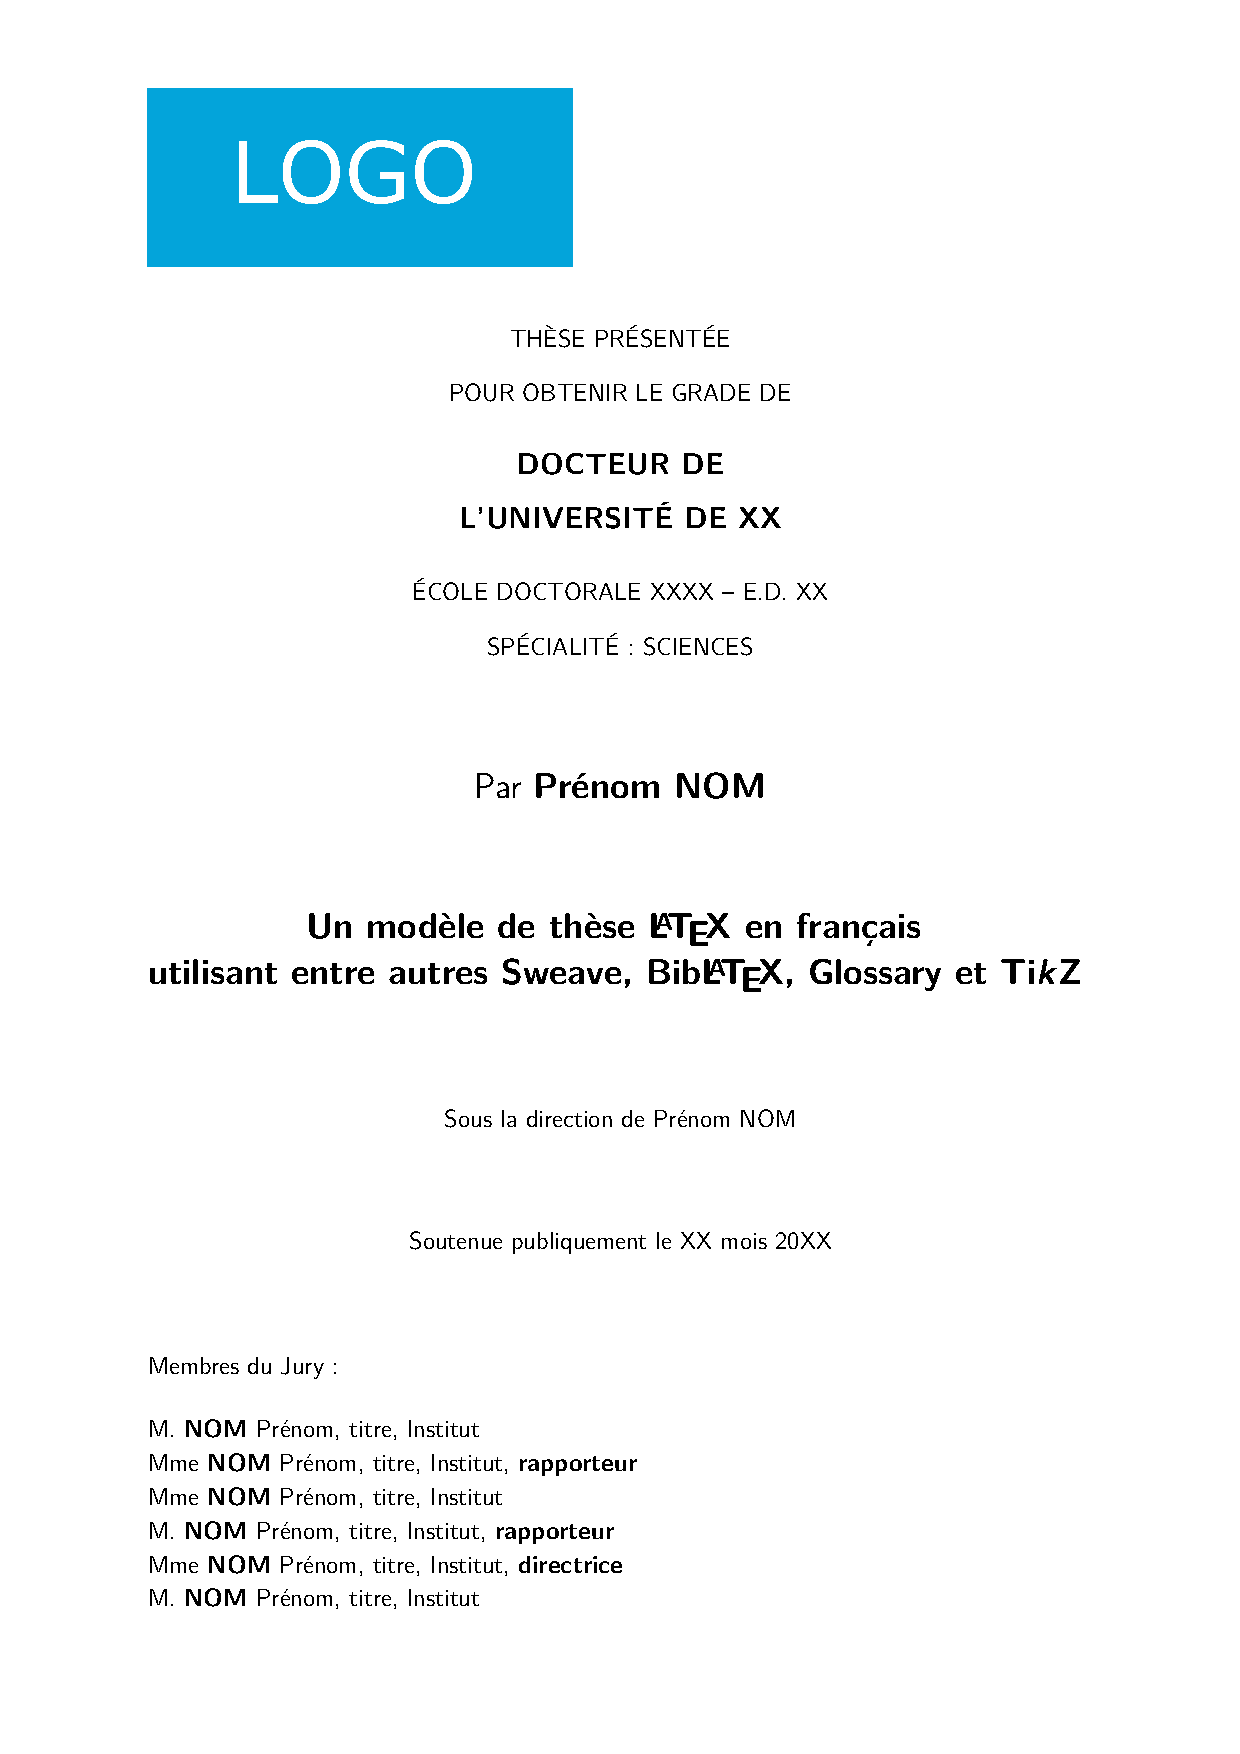
\includepdf{build/pagegarde.pdf}% fichier pagegarde.tex à compiler au préalable simplement avec pdf latex 

\setcounter{page}{1}
\cleardoublepage

%%%%%%%%
% Avertissement
\cleardoublepage 
\thispagestyle{plain}
%\phantomsection
%\addcontentsline{toc}{chapter}{Avertissement}
\hypertarget{avert}{} % Lien en métadonnées, mais pas de renvoi dans les toc
\bookmark[level=chapter,dest=avert]{Avertissement}
% Avertissement
\begin{vcenterpage}
\begin{flushleft}
\textit{L'Université n'entend ni approuver ou ni désapprouver les opinions particulières du candidat. Ces opinions doivent être considérées comme propres à leur auteur.} 
\end{flushleft}   
\end{vcenterpage}
%%%%%%%%
% Résumé
\cleardoublepage 
\thispagestyle{plain}
\hypertarget{resum}{} % Lien en métadonnées, mais pas de renvoi dans les toc
\bookmark[level=chapter,dest=resum]{Résumé\slash Abstract}
\pagestyle{empty} 

% Résumé
\begin{centerpage}
\selectlanguage{french}
\noindent {\textbf{Titre de la thèse}}
\begin{abstract} 
\noindent \lipsum[1]
\end{abstract}
{\small
\noindent {\textbf{Mots-clés:} mot-clé1, mot-clé2, mot-clé3, mot-clé4}
}

\vspace{1cm}

\hrule

\vspace{1cm}

\selectlanguage{english}
\noindent {\textbf{Thesis title}}
\begin{abstract} 
\noindent \lipsum[1]
\end{abstract}
{\small
\noindent {\textbf{Keywords:} keyword1, keyword2, keyword3, keyword4}
}

\vspace{1cm}

\hrule

\vspace{1cm}
\end{centerpage}

%%%%%%%%
% Remerciements
\cleardoublepage 
\pagestyle{plain}
\hypertarget{merci}{}% Lien en métadonnées, mais pas de renvoi dans les toc
\bookmark[level=chapter,dest=merci]{Remerciements}
%Remerciements
\chapter*{Remerciements}\markboth{\textit{Remerciements}}{}

Voici un template issu de mon manuscrit de thèse. Ce template est le résultat des ouvrages, des billets de forum, des posts de blogs de toute la communauté \R{} et \TeX{}. Merci à vous tous qui partageaient vos scripts et mettaient vos compétences au service d'une recherche diffusable et reproductible.  Si à son tour, ce template peut servir et faire gagner du temps à un doctorant j'en serais ravie. 

\begin{vcenterpage}
\begin{flushright}
\textit{Pour X. et Y.}
\end{flushright}
\end{vcenterpage}

\begingroup
\setlength{\parskip}{1pt}
%%%%%%%%
% Citation
\cleardoublepage % Affichage en page impaire (option twoside) 
\thispagestyle{plain}
\begin{vcenterpage}
\begin{flushleft}
\epigraph{"Un épigraphe pour donner le ton\dots "}{\textit{Ouvrage inconnu}\\ {\scshape Auteur inconnu}}
\end{flushleft}
\end{vcenterpage}

%%%%%%%%
% Sommaire
\cleardoublepage 
\pagestyle{plain}
\hypertarget{somcourt}{} % Lien en métadonnées, mais pas de renvoi dans les toc
\bookmark[level=chapter,dest=somcourt]{Sommaire}
% Sommaire
\shorttoc{Sommaire}{1}  % Sommaire (toc simplifié) : 2 niveaux (chapitres (0) et sections (1))
\endgroup

% Corps du document
\mainmatter
\cleardoublepage
\pagestyle{scrheadings} 

\phantomsection
\addcontentsline{toc}{chapter}{Introduction générale}
\chapter*{Introduction générale \label{chap:intro}}\markboth{Introduction générale}{Introduction générale}
%!TEX encoding = utf8

Je partage ici le \etran{template} qui a servi à la rédaction de mon manuscrit de thèse. Ce document est avant tout une sorte de patron à la rédaction d'un document long. Ce n'est pas un ouvrage dédié à \LaTeX{} même si je rappelle dans le corps du texte quelques commandes qui m'ont été très utiles. 

\begin{figure}
\renewcommand{\thefigure}{I.\arabic{figure}}
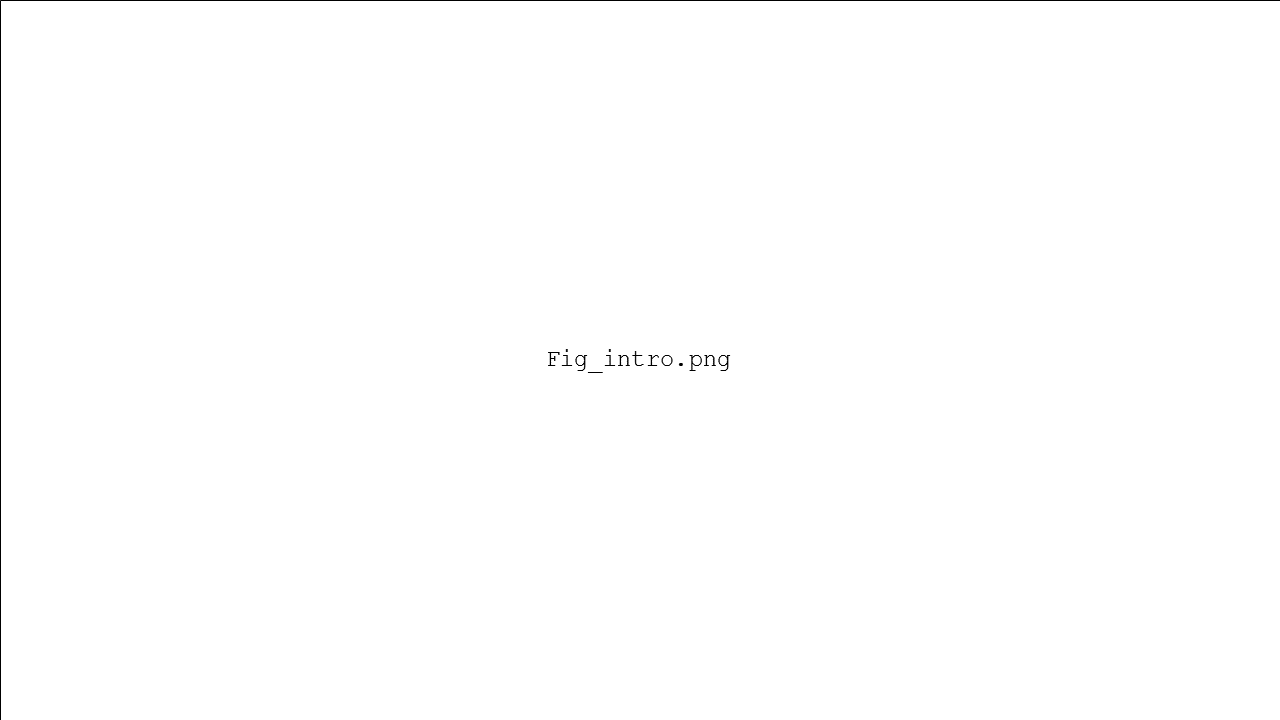
\includegraphics[width=\textwidth]{pictures/fig_intro.png}
\caption[Titre alpha court de la figure]{Titre alpha long de la figure -- avec un commentaire (source: \citetalias{DBGEOFLA})}\label{fig:intro}
\end{figure}

\section*{Classe de document et packages}

J'uilise ici la classe de document \verb!scrbook! de \verb!KOMA-script!. Pour en savoir plus, allez lire le document suivant très complet \url{https://framabook.org/docs/komascript/KOMAScript_Framaboook_LPPL.pdf}. Les packages \emph{principaux} qui sous-tendent ce document sont \verb!sweave!, \verb!siunitx!, \verb!tikz!, \verb!glossary!, \verb!biblatex! associé à \verb!natbib!, et \verb!hyperref!. L'ensemble des packages et éléments de configuration sont rassemblés dans le dossier \verb!preambule!. Pour connaitre la liste exhaustive des packages appelés, vous pouvez consulter le fichier \verb!build/these_docprincipal.log!. Notez que certains packages sont spécifiques à \verb!KOMA-script!. 

\section*{Au sujet des métadonnées}

Notez que le package \verb!hyperref! permet de spécifier les métadonnées du fichier (auteur, nom du fichier, sujet, mots-clés). N'oubliez pas de modifier ces dernières dans les fichiers \verb!pagedegarde.tex! et \verb!preambule/PDF_related.tex!. 

\section*{Autre titre non numéroté de l'introduction}

Pour obtenir une introduction suffisamment longue et ainsi avoir une idée de la mise en page, introduisons dorénavant un peu de \latin{lipsum}.

\lipsum[3-4]

\chapter[Dans le texte]{\Longstack[l]{Dans le texte: citations, références, \\ acronymes et glossaire}  \label{chap:1}}% 
%!TEX encoding = utf8
\glsresetall % réinitialisation des acronymes

\section[Titre court de la section 1]{Un exemple de titre long de la section 1 du chapitre 1}\label{sec:11}

\subsection{Sous-section 1 de la section 1}

Enumerer:
\begin{enumerate}
\item objet;
\item objet;
\item objet.
\end{enumerate}

Lister:
\begin{itemize}
\item objet;
\item objet;
\item objet.
\end{itemize}

\subsubsection{Sous-sous-section 1 de la section 1}

\paragraph{Paragraph}

\paragraph{Paragraph}

\subsubsection{Sous-sous-section 2 de la section 1}

\subsection{Sous-section 2}

\section[Des commandes dans le corps du texte]{Des commandes à garder en tête lors de l'écriture qui faciliteront grandement la mise en forme finale.
}\label{sec:12}

\subsection{Citations avec natbib et extraits}

J'utilise ici le package \verb!natbib! et les commandes \verb!\citet! pour citer au format "Auteur (Année)" tel que \citet{Anselin1990}, \verb!\citep! pour citer au format "(Auteur, Année)" tel que \citep{Holloway2007}, ou \verb! \citep[p.~12]!  pour citer un auteur et une page associée tel que \citep[p.~12]{Margeon2009}. 

J'ai particulièrement personnalisé le formatage de ma bibliographie : allz voir le fichier  \verb!preambule/biblio.tex! ainsi que les fichiers \verb!macros/bibdriver_*.tex!. 
Cela me permet de citer des livres \citep{Margeon2009,Boulay2013}, des articles de revues scientifiques  \citep{Anselin1990,Holloway2007}, des rapports institutionnels \citep{Pomel2006,Roumegoux2008}, des articles de journaux \citep{AQUI20170405,LAVIGNE20130531}, des textes juridiques \citepalias{LOI200611,DECRETLOI19350730} ou encore des bases de données \citep{DBGEOFLA,DBINSEERGP} selon mes besoins.

Notez que pour citer un extrait, on a recours parfois aux ellipses, \LaTeX{} a prévu une commande à cette fin \verb!\textellipsis! : "blablabla [\textellipsis] blablabla".

\subsection{Renvois et notes de bas de page}

Utiliser des renvois en notes de bas de page \footnote{Une note de bas de page}. Indiquer un lien vers un site \url{https://www.latex-project.org/} avec la commande \verb!\url!.

Faire référence: à des figures (figure \ref{fig:exemple}), à des pages  (voir figure \ref{fig:tikztemps} en page \pageref{fig:tikztemps}), à des tableaux (tableau \ref{tab:tabresumecourt}), à des sections (section \ref{sec:11}). 

\subsection{Acronymes avec Glossary}

Utiliser un acronyme une première fois dans le chapitre : \gls{SIG}. Utiliser une seconde fois ce même acronyme dans ce chapitre: \gls{SIG}. Utiliser cet acronyme au pluriel: \glspl{SIG}. Utiliser d'autres acronymes : \gls{GIS}, \gls{SEM}, \gls{IGN}, \gls{INSEE} qui seront ensuite repris dans la \hyperref[list:acro]{liste des acronymes} en fin de document. Certains acronymes sont associés à une définition, qui est reportée dans le \hyperref[list:gloss]{glossaire} également en fin de document.  

\subsection{Ponctuations, emphases et mots étrangers}

Ecrire des points de suspension\dots avec \verb!\dots!, renvoyer au 20\ieme siècle avec \verb!\ieme!, mettre en \emph{emphase} avec \verb!\emph!. J'ai ajouter des commandes personnelles telles que \verb!\latin! pour les locutions latines \latin{etc.} et \verb!\etran! pour les mots étrangers \etran{Hello !}
\chapter[Un peu de maths]{\Longstack[l]{Un peu de maths: nombres, \\ unités, sweave, équations \\ et tableaux} \label{chap:3}}%
%!TEX encoding = utf8
\glsresetall

Pour toute la partie mathématique, j'invite le lecteur à explorer le fichier \verb!preambule/mathematiques.tex!.

\section{Des commandes pour une mise en forme mathématique automatique}\label{sec:31}

A l'instar du chapitre \ref{chap:1}, il peut être intéressant de définir des commandes de mise en forme automatique. J'ai fait le choix par exemple de créer les commandes personnelles. Pour citer des variables dans le corps de texte, j'utilise \verb!\var!qui formate automatiquement les noms de variables: par exemple,  \var{Sepal.Length}, \var{Species}. Les commandes \verb!\na!, \verb!\nodata! et \verb!\secret! permettent de leur côté de formater des valeurs soit manquantes (l'équivalent du NA), soit inexistantes (l'équivalent du NULL), soit tues pour des raisons de secret statistique. 

Pour formater automatiquement des nombres ou des unités dans le texte (ici normes françaises), on  utilise le package \verb!siunitx!:  \SI{10000}{\hectare} (commande \verb!\SI!), \num{24.14} (commande \verb!\num! pour un nombre sans unité), \si{\km\per\second} (commande  \verb!\si! pour des unités sans valeur associée).

\section{Des équations}\label{sec:32}

Pour introduire du langage mathématique dans le corps de texte, on l'encastre entre \verb!$! et \verb!$!. Par exemple, \verb!$\delta_{p}+\rho_{p}$! donne l'expression $\delta_{p}+\rho_{p}$.

S'agissant des équations, voici un exemple de mise en forme d'une équation sur plusieurs lignes: 

\noindent\begin{minipage}{0.53\linewidth} 
\begin{equation}\label{eq:long}
\begin{split}
\ln{Y}= \alpha&+\sum_{k}(\tau_{k}.T_{k})\\
&+\sum_{i}(x_{i}.X_{i})\\
&+\varepsilon
\end{split}
\end{equation}
\end{minipage}
\hfill
\begin{minipage}{0.38\linewidth} 
{\footnotesize
Avec un commentaire sur la signification des variables par exemple : $Y$ variable à expliquer, $X$ et $T$ variables explicatives, $\tau$ et $x$ des paramètres.
}
\end{minipage}

\section{Un peu de Sweave}\label{sec:33}

Pour indiquer dans le texte une valeur calculée automatiquement et simultanément \latin{via} \R{}, on peut utiliser la commande \verb!\Sexpr!. Le nombre d'observations de la table \verb!iris! du package \verb!datasets! de R se calcule par exemple avec la commande \verb!\!\verb!Sexpr{dim(iris)[1]}!  : ce qui donne un résulat de \num{150} observations. Pour aller plus loin, on peut consulter, par exemple, le document \url{https://pbil.univ-lyon1.fr/R/pdf/tdr78.pdf}.

Vous aurez remarqué que dans ce document j'introduis parfois du code source, j'utilise pour cela la commande \verb!\verb!. L'environnement \verb!verbatim! fonctionne également très bien. 
\chapter[Flottants]{\Longstack[l]{Flottants:  encadrés, images, \\  TikZ et  tableaux} \label{chap:2}}%
%!TEX encoding = utf8
\glsresetall

Dans ce chapitre, j'ai inséré des "flottants" à savoir des encadrés courts et longs, une figure, du Ti\textit{k}Z ainsi que des tableaux. Les packages et commandes ont été déclarés dans les fichiers \verb!preambule/floating.tex! et \verb!preambule/dessin.tex!.

Par défaut, les figures sont insérées sur une pleine page (fichier: \verb!preambule/floating.tex!). 
Dans la légende de la figure \ref{fig:exemple}, j'utilise la commande personnelle \verb!\citetalias! pour citer simplement une base de données. Parfois, on peut avoir besoin d'introduire une figure sur plusieurs pages (voir figure \ref{fig:exemplelong}). On utilise alors la commande \verb!\ContinuedFloat! du package \verb!subfig!. 

J'ai inséré des figures réalisées en Ti\textit{k}Z qui m'avaient particulièrement marquées et que je m'étais réappropriées pour ma thèse. Ces figures ont été réalisées grâce à des partages de scripts de la communauté (voir fichiers du dossier \verb!tikz/!).

Enfin, j'ai inclus des tableaux (tableaux \ref{tab:tabdico} et \ref{tab:tabresumecourt}). Dans la mesure où on peut introduire un grand nombre de variables dans l'analyse, le tableau \ref{tab:tabdico} est par défaut un \verb!longtable!, ce qui lui permet de s'étendre sur plusieurs pages le cas échéant. Mais de petits tableaux tels que le tableau \ref{tab:tabresumecourt} peuvent également être plus simplement utilisés.

\section[Des encadrés]{Une section où sont insérés des encadrés courts et longs}\label{sec:21}

\lipsum[4]

\begin{frameenv}{Un encadré court}{Un encadré court}\label{enc:court}
\lipsum[1]
\end{frameenv}

\lipsum[5]

\lipsum[6]

\lipsum[7]

\begin{frameenv}{Un encadré long}{Un encadré long}\label{enc:long}
\lipsum[12-15]
\textit{(suite page \pageref{enc:long2})}
\end{frameenv}
\begin{frameenv*}{}{Un encadré long (suite)}\label{enc:long2}
\lipsum[15-19]
\end{frameenv*}

\lipsum[8]

\lipsum[9]

\section[Des figures]{Une section où sont insérés des figures}\label{sec:22}

\begin{figure}
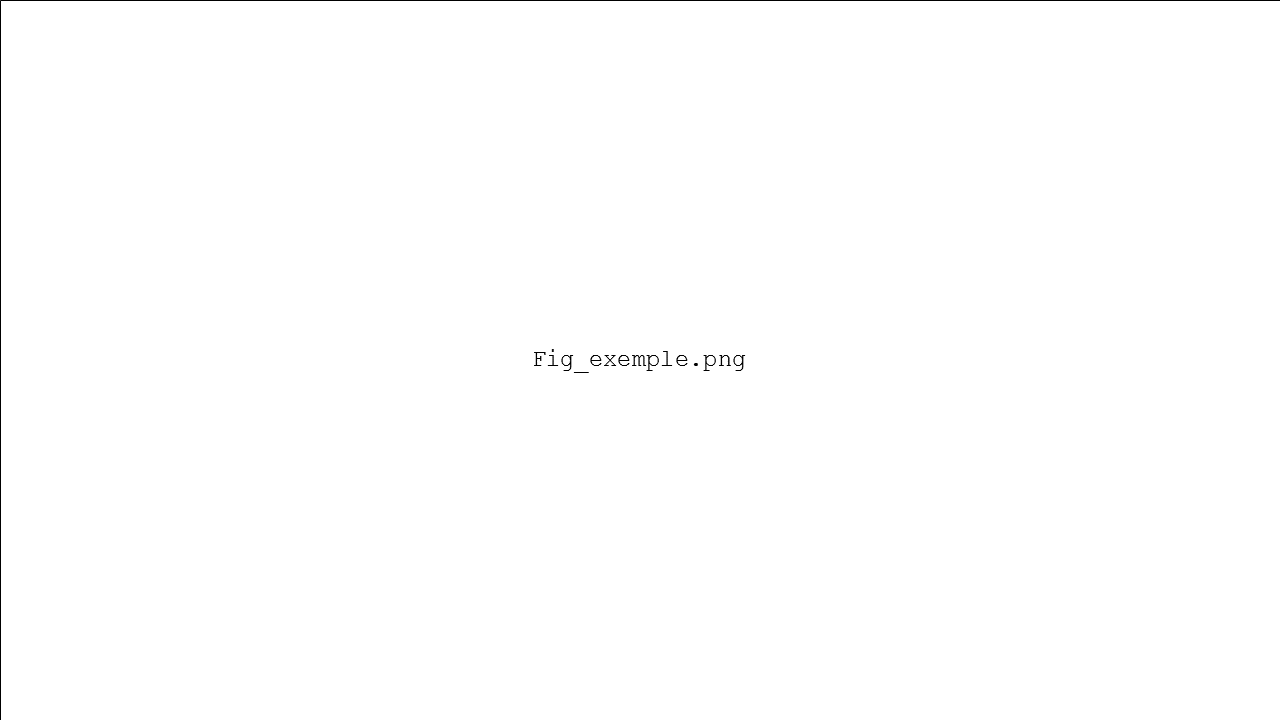
\includegraphics[width=\textwidth]{pictures/fig_exemple.png}
\caption[Titre court de la figure]{Titre long de la figure (données: \citetalias{DBINSEERGP,DBGEOFLA}; calculs et représentation graphique: l'auteur)}\label{fig:exemple}
\end{figure}

\lipsum[10]

\lipsum[11]

\lipsum[12]

\lipsum[13]

\lipsum[14]

\lipsum[15]

\begin{figure}[p]
\fbox{%
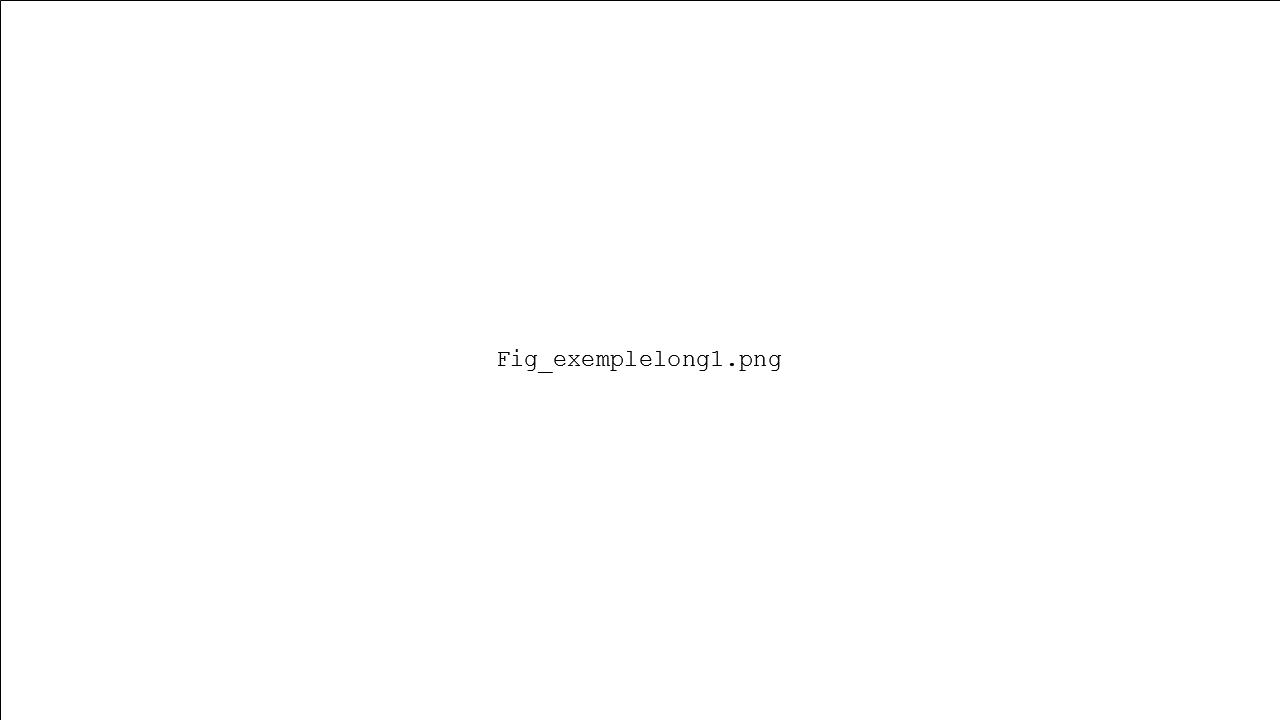
\includegraphics[page=1,width=0.95\textwidth]{pictures/fig_exemplelong1.png}}
\caption{Une illustration sur plusieurs pages}
\label{fig:exemplelong}
\end{figure}
\begin{figure}[p]
\ContinuedFloat % Suite
\captionsetup{list=no} % Non mentionné dans la liste des figures
\fbox{%
\includegraphics[page=2,width=0.95\textwidth]{pictures/fig_exemplelong2.png}}
\caption{Une illustration sur plusieurs pages (suite)}
\end{figure}

\lipsum[16]

\lipsum[17]

\lipsum[18]

\lipsum[19]

\section[Un peu de TikZ]{Une section où sont insérés des exemples de figures réalisées en TikZ}\label{sec:23}

\lipsum[18]

\lipsum[19]

\begin{figure}
\centering
% Tikz figure
% Source : http://www.texample.net/tikz/examples/gajski-kuhn-y-chart/


\scalebox{0.85}{
\begin{tikzpicture}[>=stealth',join=bevel,font=\sffamily,auto,on grid,decoration={markings,
    mark=at position .5 with \arrow{>}}]
    \coordinate (behaviouralNode) at (135:4cm);
    \coordinate (structuralNode) at (45:4cm);
    \coordinate (physicalNode) at (270:4cm);
    \coordinate (originNode) at (0:0cm);

    \node [above=1em] at (behaviouralNode) {\textbf{Behavioural Domain}};
    \node [above=1em] at (structuralNode) {\textbf{Structural Domain}};
    \node [below=1em] at (physicalNode) {\textbf{Physical Domain}};

    \draw[-, very thick] (behaviouralNode.south) -- (0,0) node[left,pos=0]{Systems} node[left,pos=0.2]{Algorithms} node[left,pos=0.4]{Register transfers} node[left,pos=0.6]{Logic} node[left,pos=0.8]{Transfer functions};

    \draw[-, very thick] (structuralNode.south) -- (0,0) node[pos=0]{ } node[pos=0.2]{Processors} node[pos=0.4]{ALUs, RAM, etc.} node[pos=0.6]{Gates, flip-flops, etc.} node[pos=0.8]{Transistors};

    \draw[-, very thick] (physicalNode.south) -- (0,0) node[right,pos=0]{Physical partitions} node[right,pos=0.2]{Floorplans} node[right,pos=0.4]{Module layout} node[right,pos=0.6]{Cell layout} node[right,pos=0.8]{Transistor layout};

    \draw[fill] (barycentric cs:behaviouralNode=1.0,originNode=0) circle (2pt);
    \draw[fill] (barycentric cs:behaviouralNode=0.8,originNode=0.2) circle (2pt);
    \draw[fill] (barycentric cs:behaviouralNode=0.6,originNode=0.4) circle (2pt);
    \draw[fill] (barycentric cs:behaviouralNode=0.4,originNode=0.6) circle (2pt);
    \draw[fill] (barycentric cs:behaviouralNode=0.2,originNode=0.8) circle (2pt);

    \draw[fill] (barycentric cs:structuralNode=1.0,originNode=0) circle (2pt);
    \draw[fill] (barycentric cs:structuralNode=0.8,originNode=0.2) circle (2pt);
    \draw[fill] (barycentric cs:structuralNode=0.6,originNode=0.4) circle (2pt);
    \draw[fill] (barycentric cs:structuralNode=0.4,originNode=0.6) circle (2pt);
    \draw[fill] (barycentric cs:structuralNode=0.2,originNode=0.8) circle (2pt);

    \draw[fill] (barycentric cs:physicalNode=1.0,originNode=0) circle (2pt);
    \draw[fill] (barycentric cs:physicalNode=0.8,originNode=0.2) circle (2pt);
    \draw[fill] (barycentric cs:physicalNode=0.6,originNode=0.4) circle (2pt);
    \draw[fill] (barycentric cs:physicalNode=0.4,originNode=0.6) circle (2pt);
    \draw[fill] (barycentric cs:physicalNode=0.2,originNode=0.8) circle (2pt);

    \draw[black!50] (0,0) circle (4.0cm);
    \draw[black!50] (0,0) circle (3.2cm);
    \draw[black!50] (0,0) circle (2.4cm);
    \draw[black!50] (0,0) circle (1.6cm);
    \draw[black!50] (0,0) circle (0.8cm);

  \end{tikzpicture}
}
\caption[Schéma TikZ: tensions]{Schéma TikZ: diagramme tensions (source: l'auteur)}\label{fig:tikztensions}
\end{figure}

\lipsum[20]

\lipsum[21]

\begin{figure}
%% Tikz figure
%% Source : https://olivierlemaire.wordpress.com/2010/12/21/frise-chronologique/ (site initial supprimé par son auteur)
%% https://fr.comp.text.tex.narkive.com/FPmUJXhp/frise-chronologique-timeline

%% commandes définies (et à personnaliser) dans le fichier macros/frise.tex
\pgfdeclarelayer{antiground}
\pgfdeclarelayer{background}
\pgfdeclarelayer{foreground}
\pgfsetlayers{antiground,background,main,foreground}

% new commands

\newcommand{\topLegend}[2]{
  node [text centered,%
  %shade,%
  %top color=\fColor,%
  %draw,%
  semithick,
  rounded corners=2pt,
  above,
  #1] {#2}}

\newcommand{\crisisLegend}[2]{
  node [text centered,%
  %shade,%
  %top color=\fColor,%
  %draw,%
  semithick,
  anchor=north,
  rounded corners=2pt,
  above,
  #1] {#2}}
  
\newcommand{\bottomLegend}[2]{
  node [text centered,%
  %shade,%
  %top color=\fColor,%
  %draw,%
  semithick,
  rounded corners=2pt,
  below,
  #1] {#2}}
  
\newcommand{\topEvent}[3]{\draw[<-,very thick,draw=lg] (#1) coordinate (#2) (#2 |- xH axis) -- ++ (#3)}
\newcommand{\bottomEvent}[3]{\draw[<-,very thick,draw=lg] (#1) coordinate (#2) (#2 |- xL axis) -- ++ (#3)}
\newcommand{\bottomGraphics}[2]{node[draw,anchor=north,inner sep=1pt,thin] {\includegraphics[#1]{#2}}}
\newcommand{\topGraphics}[2]{node[draw,anchor=south,inner sep=1pt,thin] {\includegraphics[#1]{#2}}}

\resizebox{\textwidth}{!}{%
\begin{tikzpicture}[%
=latex,%
font=\fontfamily{phv}\fontsize{7}{8}\selectfont,
legend/.style={%
draw,
rounded corners=2pt,
shade}]

% frise
\draw[rounded corners,shade,left color=blue_dark!40,right color=blue_dark!5] (-14,0) -- ++ (28,0) -- ++ (1,1.5) -- ++(-1,1.5) -- ++ (-28,0) -- cycle;
% axe bas
\path (-10,0) -- (10,0) coordinate (xL axis);
% axe haut
\path[yshift=+3cm] (-10,0) -- (10,0) coordinate (xH axis);
% rupture
\path[] (1.25,-0.25) rectangle ++(5mm,3.5) node [midway,rotate=90,minimum width=3.5cm,shade,sharp corners,inner sep=1pt] (r1) {\tiny rupture};
\draw[densely dotted] (r1.south east) -- (r1.south west) (r1.north east) -- (r1.north west);
\draw[] (0,0) coordinate (an0) -- (an0 |- xH axis) -- ++ (0,2.5mm) node [above] {An 0};


% scope 1
\begin{scope}[xshift=3cm,xscale={14cm/400cm}]
% graduation
\draw[] (0,0) coordinate (an0) -- (an0 |- xH axis) -- ++ (0,2.5mm) node [above] {1600};
\draw[] (100,0) coordinate (an100) -- (an100 |- xH axis) -- ++ (0,2.5mm) node [above] {1700};
\draw[] (200,0) coordinate (an200) -- (an200 |- xH axis) -- ++ (0,2.5mm) node [above] {1800};

% evennement
\bottomEvent{42,0}{an1642}{0,-5mm} \bottomLegend{text width=2cm,name=p}{1642 :\\Pascaline};
\topEvent{17,0}{an1617}{0,1} \topLegend{text width=4cm,name=r}{1617 :\\Napier : invention logarithmes\\W. Oughtred : R\`egles \`a calculer};
\bottomEvent{127,0}{an1727}{0,-5mm} \bottomLegend{text width=2cm}{1727 :\\Carte Perfor\'ee};
\topEvent{233,0}{an1617}{0,1} \topLegend{text width=4cm}{1833 :\\machine \`a babbage\\1ere Programmeuse : A. Lovelace};
\end{scope}

% scope 2
\begin{scope}[xshift=0cm,xscale={0.7cm/30cm}]
% graduation
\draw[] (-100,0) coordinate (anM1000) -- (anM1000 |- xH axis) -- ++ (0,2.5mm) node [above,fill=white] {-1000};
\draw[] (-200,0) coordinate (anM2000) -- (anM2000 |- xH axis) -- ++ (0,2.5mm) node [above,fill=white] {-2000};
\draw[] (-300,0) coordinate (anM3000) -- (anM3000 |- xH axis) -- ++ (0,2.5mm) node [above,fill=white] {-3000};
%evennement
\bottomEvent{-30,0}{anM300}{0,-5mm} \bottomLegend{text width=2.5cm}{-300 :\\Abaques et bouliers};
\topEvent{-30,0}{anM3002}{0,2cm} \topLegend{text width=4cm}{-300 : logique\\syllogismes (\textsc{socrates})\\
\vspace{-12pt}\begin{enumerate}\itemsep-2pt
\item tout homme est mortel
\item or Socrates est un homme
\item donc Socrates est mortel
\end{enumerate}
};
\topEvent{-173,0}{anM1730}{0,7.5mm} \topLegend{text width=2.5cm}{-1730 :\\1er algorithme};
\bottomEvent{-300,0}{anM1730}{0,-5mm} \bottomLegend{text width=3.5cm}{-3000 :\\apparition du binaire dans le symbole de l'empereur chinois Fou~Hi};
\end{scope}
\end{tikzpicture}
}
\caption[Schéma TikZ: chronologie]{Schéma TikZ: chronologie (source: l'auteur) 
\comment{La frise chronologique n'a pas vocation à être exhaustive. Les dates indiquées sont celles mentionnées dans le texte.}}\label{fig:tikztemps}
\end{figure}

\begin{figure}
%% Tikz figure
%% Source : http://www.texample.net/tikz/examples/swan-wave-model/

\resizebox{\textwidth}{!}{%
\begin{tikzpicture}[scale=.9,every node/.style={minimum size=1cm},on grid]
		
    %slanting: production of a set of n 'laminae' to be piled up. N=number of grids.
    \begin{scope}[
            yshift=-83,every node/.append style={
            yslant=0.5,xslant=-1},yslant=0.5,xslant=-1
            ]
        % opacity to prevent graphical interference
        \fill[white,fill opacity=0.9] (0,0) rectangle (5,5);
        \draw[step=4mm, black] (0,0) grid (5,5); %defining grids
        \draw[step=1mm, red!50,thin] (3,1) grid (4,2);  %Nested Grid
        \draw[black,very thick] (0,0) rectangle (5,5);%marking borders
        \fill[red] (0.05,0.05) rectangle (0.35,0.35);
        %Idem as above, for the n-th grid:
    \end{scope}
    	
    \begin{scope}[
    	yshift=0,every node/.append style={
    	    yslant=0.5,xslant=-1},yslant=0.5,xslant=-1
    	             ]
        \fill[white,fill opacity=.9] (0,0) rectangle (5,5);
        \draw[black,very thick] (0,0) rectangle (5,5);
        \draw[step=5mm, black] (0,0) grid (5,5);
    \end{scope}
    	
    \begin{scope}[
    	yshift=90,every node/.append style={
    	yslant=0.5,xslant=-1},yslant=0.5,xslant=-1
    	             ]
    	\fill[white,fill opacity=.9] (0,0) rectangle (5,5);
    	\draw[step=10mm, black] (1,1) grid (4,4);
    	\draw[black,very thick] (1,1) rectangle (4,4);
    	\draw[black,dashed] (0,0) rectangle (5,5);
    \end{scope}
    	
    \begin{scope}[
    	yshift=170,every node/.append style={
    	    yslant=0.5,xslant=-1},yslant=0.5,xslant=-1
    	  ]
        \fill[white,fill opacity=0.6] (0,0) rectangle (5,5);
        \draw[step=10mm, black] (2,2) grid (5,5);
        \draw[step=2mm, green] (2,2) grid (3,3);
        \draw[black,very thick] (2,2) rectangle (5,5);
        \draw[black,dashed] (0,0) rectangle (5,5);
    \end{scope}
    	
    \begin{scope}[
        yshift=-170,every node/.append style={
        yslant=0.5,xslant=-1},yslant=0.5,xslant=-1
                  ]
        %marking border
        \draw[black,very thick] (0,0) rectangle (5,5);

       	%drawing corners (P1,P2, P3): only 3 points needed to define a plane.
        \draw [fill=lime](0,0) circle (.1) ;
        \draw [fill=lime](0,5) circle (.1);
        \draw [fill=lime](5,0) circle (.1);
        \draw [fill=lime](5,5) circle (.1);

        %drawing bathymetric hypotetic countours on the bottom grid:    	
        \draw [ultra thick](0,1) parabola bend (2,2) (5,1)  ;
        \draw [dashed] (0,1.5) parabola bend (2.5,2.5) (5,1.5) ;
        \draw [dashed] (0,2) parabola bend (2.7,2.7) (5,2)  ;
        \draw [dashed] (0,2.5) parabola bend (3.5,3.5) (5,2.5)  ;
        \draw [dashed] (0,3.5)  parabola bend (2.75,4.5) (5,3.5);
        \draw [dashed] (0,4)  parabola bend (2.75,4.8) (5,4);
        \draw [dashed] (0,3)  parabola bend (2.75,3.8) (5,3);
        \draw[-latex,thick](2.8,1)node[right]{$\mathsf{Shoreline}$}
                 to[out=180,in=270] (2,1.99);
    \end{scope} %end of drawing grids

    %putting arrows and labels:
    \draw[-latex,thick] (6.2,2) node[right]{$\mathsf{Bathymetry}$}
         to[out=180,in=90] (4,2);

    \draw[-latex,thick](5.8,-.3)node[right]{$\mathsf{Comp.\ G.}$}
        to[out=180,in=90] (3.9,-1);

    \draw[-latex,thick](5.9,5)node[right]{$\mathsf{Wind\ G.}$}
        to[out=180,in=90] (3.6,5);

    \draw[-latex,thick](5.9,8.4)node[right]{$\mathsf{Friction\ G.}$}
        to[out=180,in=90] (3.2,8);

    \draw[-latex,thick,red](5.3,-4.2)node[right]{$\mathsf{G. Cell}$}
        to[out=180,in=90] (0,-2.5);

    \draw[-latex,thick,red](4.3,-1.9)node[right]{$\mathsf{Nested\ G.}$}
        to[out=180,in=90] (2,-.5);

    \draw[-latex,thick](4,-6)node[right]{$\mathsf{Batymetry}$}
        to[out=180,in=90] (2,-5);	
    %drawing points on grid's conrners.
    \fill[black,font=\footnotesize]
        (-5,-4.3) node [above] {$P_{1}$}
        (-.3,-5.6) node [below] {$P_{2}$}
        (5.5,-4) node [above] {$P_{3}$};	
\end{tikzpicture}}
\caption[Schéma TikZ: multi-échelles]{Schéma TikZ: multi-échelles (source: l'auteur)}\label{fig:tikzsources}
\end{figure}

\lipsum[22]

\lipsum[23]

\section[Des tableaux ]{Des tableaux}\label{sec:24}

\lipsum[24]

\begin{table}
\caption{Résumé numérique des variables de la table iris (tableau simple)} \label{tab:tabresumecourt}
\begin{tabular}{lcrrrrr}
\toprule 
& Unité & Min & $\widetilde{x}$ & $\bar{x}$ & Max & $\sigma_{x}$ \\ 
\midrule 
\var{Sepal.Length} &  \si{\cm} \num{4.3} & \num{5.8} & \num{5.8} & \num{7.9} & \num{0.8} \\ 
\var{Sepal.Width} &  \si{\cm} & \num{2.0} & \num{3.0} & \num{3.1} & \num{4.4} & \num{0.4} \\ 
\var{Petal.Length} &  \si{\cm} & \num{1.0} & \num{4.3} & \num{3.8} & \num{6.9} & \num{1.8} \\ 
\var{Petal.Width} &  \si{\cm} & \num{0.1} & \num{1.3} & \num{1.2} & \num{2.5} & \num{0.8} \\ 
\var{Species} &  - & \nodata{} & \nodata{} & \nodata{} & \nodata{} & \nodata{}\\ 
\bottomrule 
\end{tabular}
\end{table}

\lipsum[25]

\begin{longtable}{>{\raggedright}p{.18\linewidth}p{.16\linewidth}p{.522\linewidth}}%
%
\caption{Définition des variables introduites dans le modèle} \label{tab:tabdico}\\
\toprule
Source & Variable & Définition\\
\midrule 
\endfirsthead 
%
\caption[]{Définition des variables introduites dans le modèle (suite)}\\
\toprule 
Source & Variable & Définition\\
\midrule
\endhead 
%
\midrule
\textit{Suite page suivante}
\endfoot 
%
\bottomrule
\notelinespace
\textit{Note:} & \multicolumn{2}{r}{} 
\endlastfoot 
%
R dataset iris & \var{Sepal.Length} & Longueur des sépales en \si{\cm} \\ 
& \var{Sepal.Width} & Largeur des sépales en \si{\cm} \\ 
& \var{Petal.Length} & Longueur des pétales en \si{\cm} \\ 
& \var{Petal.Width} & Largeur des pétales en \si{\cm} \\ 
& \var{Species} & Nom de l'espère \\ 
\addlinespace
R dataset CO2 & \var{Plant} & Identifiant de chaque plante \\ 
& \var{Type} & Origine de la plante \\ 
& \var{conc} & Concentration ambiante en dioxyde de carbone en \si{\ml\per\L}\\
& \var{uptake} & Taux d'absorption en \si{\umol\m\squared\per\second)}\\
R dataset iris & \var{Sepal.Length} & Longueur des sépales en \si{\cm} \\ 
& \var{Sepal.Width} & Largeur des sépales en \si{\cm} \\ 
& \var{Petal.Length} & Longueur des pétales en \si{\cm} \\ 
& \var{Petal.Width} & Largeur des pétales en \si{\cm} \\ 
& \var{Species} & Nom de l'espère \\ 
\addlinespace
R dataset CO2 & \var{Plant} & Identifiant de chaque plante \\ 
& \var{Type} & Origine de la plante \\ 
& \var{conc} & Concentration ambiante en dioxyde de carbone en \si{\ml\per\L}\\
& \var{uptake} & Taux d'absorption en \si{\umol\m\squared\per\second)}\\
R dataset iris & \var{Sepal.Length} & Longueur des sépales en \si{\cm} \\ 
& \var{Sepal.Width} & Largeur des sépales en \si{\cm} \\ 
& \var{Petal.Length} & Longueur des pétales en \si{\cm} \\ 
& \var{Petal.Width} & Largeur des pétales en \si{\cm} \\ 
& \var{Species} & Nom de l'espère \\ 
\addlinespace
R dataset CO2 & \var{Plant} & Identifiant de chaque plante \\ 
& \var{Type} & Origine de la plante \\ 
& \var{conc} & Concentration ambiante en dioxyde de carbone en \si{\ml\per\L}\\
& \var{uptake} & Taux d'absorption en \si{\umol\m\squared\per\second)}\\
R dataset iris & \var{Sepal.Length} & Longueur des sépales en \si{\cm} \\ 
& \var{Sepal.Width} & Largeur des sépales en \si{\cm} \\ 
& \var{Petal.Length} & Longueur des pétales en \si{\cm} \\ 
& \var{Petal.Width} & Largeur des pétales en \si{\cm} \\ 
& \var{Species} & Nom de l'espère \\ 
\addlinespace
R dataset CO2 & \var{Plant} & Identifiant de chaque plante \\ 
& \var{Type} & Origine de la plante \\ 
& \var{conc} & Concentration ambiante en dioxyde de carbone en \si{\ml\per\L}\\
& \var{uptake} & Taux d'absorption en \si{\umol\m\squared\per\second)}\\
R dataset iris & \var{Sepal.Length} & Longueur des sépales en \si{\cm} \\ 
& \var{Sepal.Width} & Largeur des sépales en \si{\cm} \\ 
& \var{Petal.Length} & Longueur des pétales en \si{\cm} \\ 
& \var{Petal.Width} & Largeur des pétales en \si{\cm} \\ 
& \var{Species} & Nom de l'espère \\ 
\addlinespace
R dataset CO2 & \var{Plant} & Identifiant de chaque plante \\ 
& \var{Type} & Origine de la plante \\ 
& \var{conc} & Concentration ambiante en dioxyde de carbone en \si{\ml\per\L}\\
& \var{uptake} & Taux d'absorption en \si{\umol\m\squared\per\second)}\\
R dataset iris & \var{Sepal.Length} & Longueur des sépales en \si{\cm} \\ 
& \var{Sepal.Width} & Largeur des sépales en \si{\cm} \\ 
& \var{Petal.Length} & Longueur des pétales en \si{\cm} \\ 
& \var{Petal.Width} & Largeur des pétales en \si{\cm} \\ 
& \var{Species} & Nom de l'espère \\ 
\addlinespace
R dataset CO2 & \var{Plant} & Identifiant de chaque plante \\ 
& \var{Type} & Origine de la plante \\ 
& \var{conc} & Concentration ambiante en dioxyde de carbone en \si{\ml\per\L}\\
& \var{uptake} & Taux d'absorption en \si{\umol\m\squared\per\second)}\\
\end{longtable}

\cleardoublepage 
\phantomsection
\addcontentsline{toc}{chapter}{Conclusion générale}
\chapter*{Conclusion générale \label{chap:conclu}}\markboth{Conclusion générale}{Conclusion générale}
\lipsum[5-6]

% Appendix
\appendix
\cleardoublepage 
%%%%%%%%%%%%%%
% Annexes personnalisées
\addchap[Annexes]{Annexes}

\renewcommand\thefigure{A.\alph{figure}}   % Numérotation alpha des figures
\setcounter{figure}{0} % Remise à niveau
\renewcommand\thetable{A.\alph{table}}   % Numérotation alpha des figures
\setcounter{table}{0} % Remise à niveau

\addsec[Packages utilisés]{Liste des packages utilisés dans ce document}
\label{app:packages}
\printfilelist

\addsec[Précisions méthologiques]{Précisions méthologiques}
\label{app:methode}
Un texte simple apportant des précisions latines sur la méthode en annexe. 
\lipsum[1-2]


% Backmatter
\backmatter
\cleardoublepage 
\pagestyle{scrheadings} 
%%%%%%%%%%%%%
% Appareil de référence
\begingroup
\setlength{\parskip}{1pt}
% Bibliographie
\cleardoubleemptypage % Nécessaire pour que le lien via hyperref se fasse correctement 
% Bibliographie
\phantomsection
\addcontentsline{toc}{chapter}{Références} % Doit être indiqué juste avant la section que l'on veut faire apparaitre dans le TOC
\printbibheading[heading=ref]
\phantomsection
\addcontentsline{toc}{section}{Ouvrages et publications académiques} 
\printbibliography[heading=subbibliography,filter=filtrescience,title={Ouvrages et publications académiques} ]
\phantomsection
\addcontentsline{toc}{section}{Publications institutionnelles} 
\printbibliography[heading=subbibliography,filter=filtrerapport,title=Publications d'organismes institutionnels]
\phantomsection
\addcontentsline{toc}{section}{Textes juridiques} 
\printbibliography[heading=subbibliography,type=legislation,title=Textes juridiques]
\phantomsection
\addcontentsline{toc}{section}{Articles de presse} 
\printbibliography[type=newspaper,heading=subbibliography,title=Articles de presse]
\phantomsection
\addcontentsline{toc}{section}{Bases de données} 
\printbibliography[type=database,heading=subbibliography,title=Bases de données]
\phantomsection
\addcontentsline{toc}{section}{Documentation technique} 
\defbibnote{prenote}{Cette pré-note me permet de préciser que les analyses économétriques et les représentations graphiques ont été réalisées avec le logiciel \R{} \citep{RTeam2012} et les extensions publiées par la communauté. Le document final a été composé avec \hologo{LaTeX} à l'aide des ouvrages de \citet{Rouquette2012,Lozano2008,Tisseau2015} et de l'ensemble de la communauté \hologo{TeX}.}
%
\nocite{Rouquette2012,Lozano2008,Tisseau2015} % rédaction
\nocite{RTeam2012}%R
\nocite{Dray2007, Maechler2014, Zeiles2002, Lewin-Koh2011, Hastie2011, Muggeo2008,Bivand2012} % Packages de la thèse

\printbibliography[heading=subbibliography, prenote=prenote,filter=filtreoutils,title=Documentation technique]

% Acronymes
\cleardoublepage % Nécessaire pour que le lien via hyperref se fasse correctement 
% Acronymes
\phantomsection
\addcontentsline{toc}{chapter}{Liste des acronymes et abréviations}\label{list:acro}
\printglossary[title=Liste des acronymes et abréviations,type=\acronymtype]

% Glossaire et Index
% Glossaire
\cleardoublepage % Affichage en page impaire (option twoside)
\phantomsection
\addcontentsline{toc}{chapter}{Glossaire}\label{list:gloss}
\printglossary[title=Glossaire]

% Tables
% Tables des figures et tableaux
\cleardoublepage % Nécessaire pour que le lien via hyperref se fasse correctement 
% Tables des figures et tableaux
\phantomsection
\addcontentsline{toc}{chapter}{Table des illustrations} % toc
\chapter*{Table des illustrations}
\phantomsection
\addcontentsline{toc}{section}{Figures} \label{list:fig}% toc
\listoffigures
\phantomsection
\addcontentsline{toc}{section}{Tableaux} \label{list:tab}% toc
\listoftables
\phantomsection
\addcontentsline{toc}{section}{Encadrés} \label{list:enc}% toc
\listofmyfloats % encadrés
% Tables des matières (toc)
\cleardoublepage % Nécessaire pour que le lien via hyperref se fasse correctement 
% Tables des matières (toc)
\phantomsection
\addcontentsline{toc}{chapter}{Table des matières} % Doit être indiqué juste avant la section que l'on veut faire apparaitre dans le TOC
\setcounter{tocdepth}{10} % Nombre de niveaux affichés dans le toc
\tableofcontents% Table des matières (TOC) détaillée (plusieurs niveaux !!)

\endgroup

\end{document}
